\documentclass[]{article}
\usepackage{lmodern}
\usepackage{amssymb,amsmath}
\usepackage{ifxetex,ifluatex}
\usepackage{fixltx2e} % provides \textsubscript
\ifnum 0\ifxetex 1\fi\ifluatex 1\fi=0 % if pdftex
  \usepackage[T1]{fontenc}
  \usepackage[utf8]{inputenc}
  \usepackage{eurosym}
\else % if luatex or xelatex
  \ifxetex
    \usepackage{mathspec}
  \else
    \usepackage{fontspec}
  \fi
  \defaultfontfeatures{Ligatures=TeX,Scale=MatchLowercase}
  \newcommand{\euro}{€}
\fi
% use upquote if available, for straight quotes in verbatim environments
\IfFileExists{upquote.sty}{\usepackage{upquote}}{}
% use microtype if available
\IfFileExists{microtype.sty}{%
\usepackage{microtype}
\UseMicrotypeSet[protrusion]{basicmath} % disable protrusion for tt fonts
}{}
\usepackage[unicode=true]{hyperref}
\hypersetup{
            pdfborder={0 0 0},
            breaklinks=true}
\urlstyle{same}  % don't use monospace font for urls
\usepackage{longtable,booktabs}
% Fix footnotes in tables (requires footnote package)
\IfFileExists{footnote.sty}{\usepackage{footnote}\makesavenoteenv{long table}}{}
\usepackage{graphicx,grffile}
\makeatletter
\def\maxwidth{\ifdim\Gin@nat@width>\linewidth\linewidth\else\Gin@nat@width\fi}
\def\maxheight{\ifdim\Gin@nat@height>\textheight\textheight\else\Gin@nat@height\fi}
\makeatother
% Scale images if necessary, so that they will not overflow the page
% margins by default, and it is still possible to overwrite the defaults
% using explicit options in \includegraphics[width, height, ...]{}
\setkeys{Gin}{width=\maxwidth,height=\maxheight,keepaspectratio}
\IfFileExists{parskip.sty}{%
\usepackage{parskip}
}{% else
\setlength{\parindent}{0pt}
\setlength{\parskip}{6pt plus 2pt minus 1pt}
}
\setlength{\emergencystretch}{3em}  % prevent overfull lines
\providecommand{\tightlist}{%
  \setlength{\itemsep}{0pt}\setlength{\parskip}{0pt}}
\setcounter{secnumdepth}{0}
% Redefines (sub)paragraphs to behave more like sections
\ifx\paragraph\undefined\else
\let\oldparagraph\paragraph
\renewcommand{\paragraph}[1]{\oldparagraph{#1}\mbox{}}
\fi
\ifx\subparagraph\undefined\else
\let\oldsubparagraph\subparagraph
\renewcommand{\subparagraph}[1]{\oldsubparagraph{#1}\mbox{}}
\fi

% set default figure placement to htbp
\makeatletter
\def\fps@figure{htbp}
\makeatother


\date{}

\begin{document}

\textbf{\emph{LE DIPENDENZE PATOLOGICHE:}}

NB: il professore riferisce che all'esame chiedono a grandi linee questi
argomenti, senza entrare eccessivamente nei dettagli

Si fa riferimento al DSM, il manuale diagnostico di psichiatria, volume
dove vengono indicati tutti i disturbi e le linee guida per la diagnosi.

Il DSM IV (penultimo uscito) divide i disturbi da sostanze in:

\begin{itemize}
\item
  \begin{quote}
  disturbi da uso di sostanze:
  \end{quote}

  \begin{itemize}
  \item
    \begin{quote}
    dipendenza
    \end{quote}
  \item
    \begin{quote}
    abuso
    \end{quote}
  \end{itemize}
\item
  \begin{quote}
  disturbi indotti da sostanze:
  \end{quote}

  \begin{itemize}
  \item
    \begin{quote}
    intossicazione
    \end{quote}
  \item
    \begin{quote}
    astinenza
    \end{quote}
  \item
    \begin{quote}
    disturbi psichici legati all'uso di sostanze
    \end{quote}
  \end{itemize}
\end{itemize}

\textbf{\emph{DEFINIZIONE DI DIPENDENZA:}}

Modalità patologica di uso della sostanza, per almeno un anno, che
conduce ad un disagio clinicamente significativo, manifestato dai
seguenti criteri:

\begin{itemize}
\item
  \begin{quote}
  tolleranza
  \end{quote}
\item
  \begin{quote}
  astinenza
  \end{quote}
\item
  \begin{quote}
  modalità compulsiva
  \end{quote}
\end{itemize}

Il criterio di esclusione (come per ogni altra patologia psichiatrica
descritta nel DSM) è che non ci sia un'altra condizione medica generale
o un altro disturbo mentale.

\begin{itemize}
\item
  \textbf{\emph{TOLLERANZA}:} bisogno di dosi sempre più elevate per
  raggiungere l'intossicazione e l'effetto desiderato (l'effetto è
  notevolmente diminuito con la stessa dose della sostanza).
\end{itemize}

\begin{quote}
E' un fenomeno di adattamento, su base biochimica.

Esiste anche il fenomeno della \textbf{cross-tolleranza}: la tolleranza
si sviluppa anche per tutte quelle sostanze che agiscono sullo stesso
recettore.

Es. un eroinomane è tollerante a tutte quelle sostanze che agiscono sul
recettore degli oppioidi come codeina, morfina, metadone; un alcolista
tollererà meglio un sedativo-ipnotico rispetto ad un soggetto astemio o
non alcolista (agiscono tutti e due sul GABA A).
\end{quote}

\begin{itemize}
\item
  \textbf{\emph{ASTINENZA}}: sindrome sostanza-specifica per diminuzione
  o cessazione di una sostanza assunta in modo prolungato.
\end{itemize}

\begin{quote}
Per definire una crisi d'astinenza il disagio deve essere significativo
e compromettere la funzionalità normale (non deve essere prodotta da
altre patologie sia organiche che psichiatriche).

L'intensità è inversamente proporzionale all'emivita della sostanza
d'abuso, invece la durata è direttamente proporzionale.
\end{quote}

L'astinenza è ciò che spinge il tossicodipendente a continuare ad
assumere la sostanza. 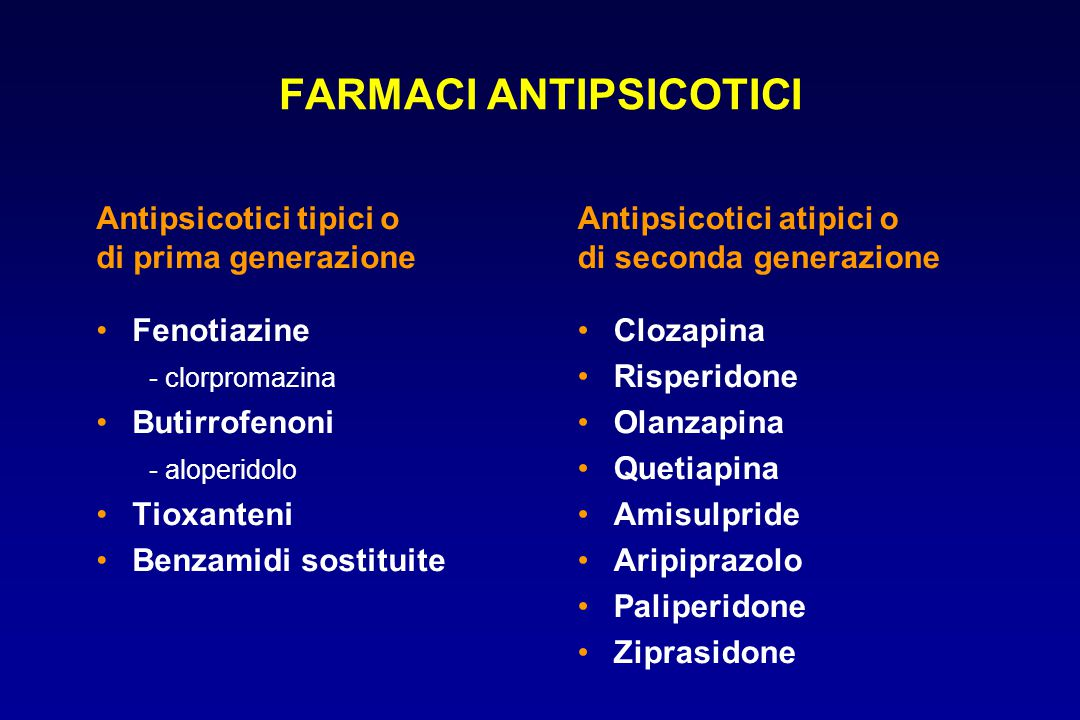
\includegraphics{media/image1.emf}

\begin{itemize}
\item
  \textbf{\emph{MODALITA' COMPULSIVA}}: \emph{craving. }
\end{itemize}

\begin{quote}
La vita del tossicodipendente diviene improntata sulla ricerca e
l'assunzione della sostanza.

La sostanza è assunta in quantità maggiore rispetto a quello che viene
previsto dal soggetto (\emph{binge} o ``abbuffata di sostanza'').

Ricerca della cosiddetta \emph{luna di miele,} ovvero la sensazione
provata con la prima assunzione.

Per dire che una persona è dipendente deve essere presente il desiderio
persistente e i tentativi infruttuosi di ridurre e controllare l'uso
della sostanza.

Nonostante siano consci di avere un dipendenza e dei danni prodotti
dalla sostanza, continuano ugualmente a ricercarla e ad assumerla.
\end{quote}

La diagnosi di dipendenza viene effettuata se il soggetto riporta le 3
caratteristiche.

\textbf{\emph{DEFINIZIONE DI ABUSO:}}

Modalità patologica di uso della sostanza, per almeno un anno, che porta
ad un disagio clinicamente significativo, non essendo però presenti le
tre caratteristiche della dipendenza.

L'uso della sostanza deve essere ricorrente e deve impedire lo
svolgimento della vita normale del soggetto (non va a lavorare, non va a
scuola, ecc...).

Il soggetto si mette a rischio a causa della sostanza (problemi legali,
rischi fisici per sé e per gli altri).

Per l'abuso è importante l'interazione tra soggetto, sostanza e
ambiente.

\textbf{\emph{DIFFERENZA TRA DIPENDENZA E ABUSO}}

\begin{longtable}[]{@{}ll@{}}
\toprule
\textbf{DIPENDENZA} & \textbf{ABUSO}\tabularnewline
Diagnosi biologica effettuata dal soggetto che, come osservatore
interno, è conscio della sua dipendenza. & Diagnosi comportamentale
eseguita dallo psichiatria, su base clinica.\tabularnewline
Caratterizzata dal rinforzo negativo (si assume la sostanza per evitare
o eliminare la crisi d'astinenza) & Caratterizzata dal rinforzo positivo
(il piacere provato dall'assunzione della sostanza)\tabularnewline
Il dipendente ha molta ansia anticipatoria prima dell'assunzione, per
evitare l'astinenza e quindi il rinforzo negativo. Quando prende la
sostanza ha una sorta di sollievo, e, non prova il senso di colpa;
avendo fatto passare o avendo evitato l'astinenza il dipendente è in
pace con se stesso. & L'abusatore è più probabile che non abbia l'ansia
anticipatoria ma che dopo abbia il senso di colpa.\tabularnewline
Interazione a 2: soggetto-sostanza & Interazione a 3:
soggetto-sostanza-ambiente\tabularnewline
COMPULSIONE → pattern di assunzione della sostanza rigido, ripetitivo,
schematico, e ha la finalità di evitare un danno. & IMPULSO → assunzione
reiterata, frequenza variabile, ed è unicamente finalizzato alla ricerca
della gratificazione.\tabularnewline
Egodistonico (costrizione all'assunzione) & Egosintonico (desiderio di
assunzione)\tabularnewline
\bottomrule
\end{longtable}

In generale il nostro cervello tende all'omeostasi, avviene il così
detto neuro adattamento. Quando si abusa di una sostanza si sposta
l'equilibrio verso un lato, quando la sostanza smette di funzionare si
avrà il disequilibrio spostato dall'altra parte.

Abuso e astinenza sono in sostanza le due facce di una medaglia.

Es. con l'assunzione di cocaina dopo la fase di eccitazione iniziale si
avrà una fase depressiva, determinata dal completo svuotamento delle
vescicole sinaptiche adrenergiche.

Questa distinzione tra dipendenza e abuso è importante dal punto di
vista clinico più che patologico.

DSM V (la nuova revisione) ha eliminato la differenza tra abuso e
dipendenza, riunendo tutto sotto il nome di ``\textbf{disturbo da uso di
sostanze}''; è appropriato mantenere la divisione poichè si
differenziano per quanto riguarda la terapia.

\textbf{\emph{NEUROBIOLOGIA}}

Il cervello si sviluppa, da un punto di vista evoluzionistico, in
direzione ventri-dorsale e medio-laterale. Le aree ventri-mediali (più
antiche) sono le fautrici del loop della dipendenza; per questo motivo
possiamo ritrovare anche in animali, come il topo, gli stessi
comportamenti di un essere umano riguardo all'uso di sostanze
stupefacenti.

Le aree ventri-mediali presentano le vie della dopamina,
neurotrasmettitore implicato nella genesi delle dipendenze.

Ci sono 4 vie dopaminergiche:

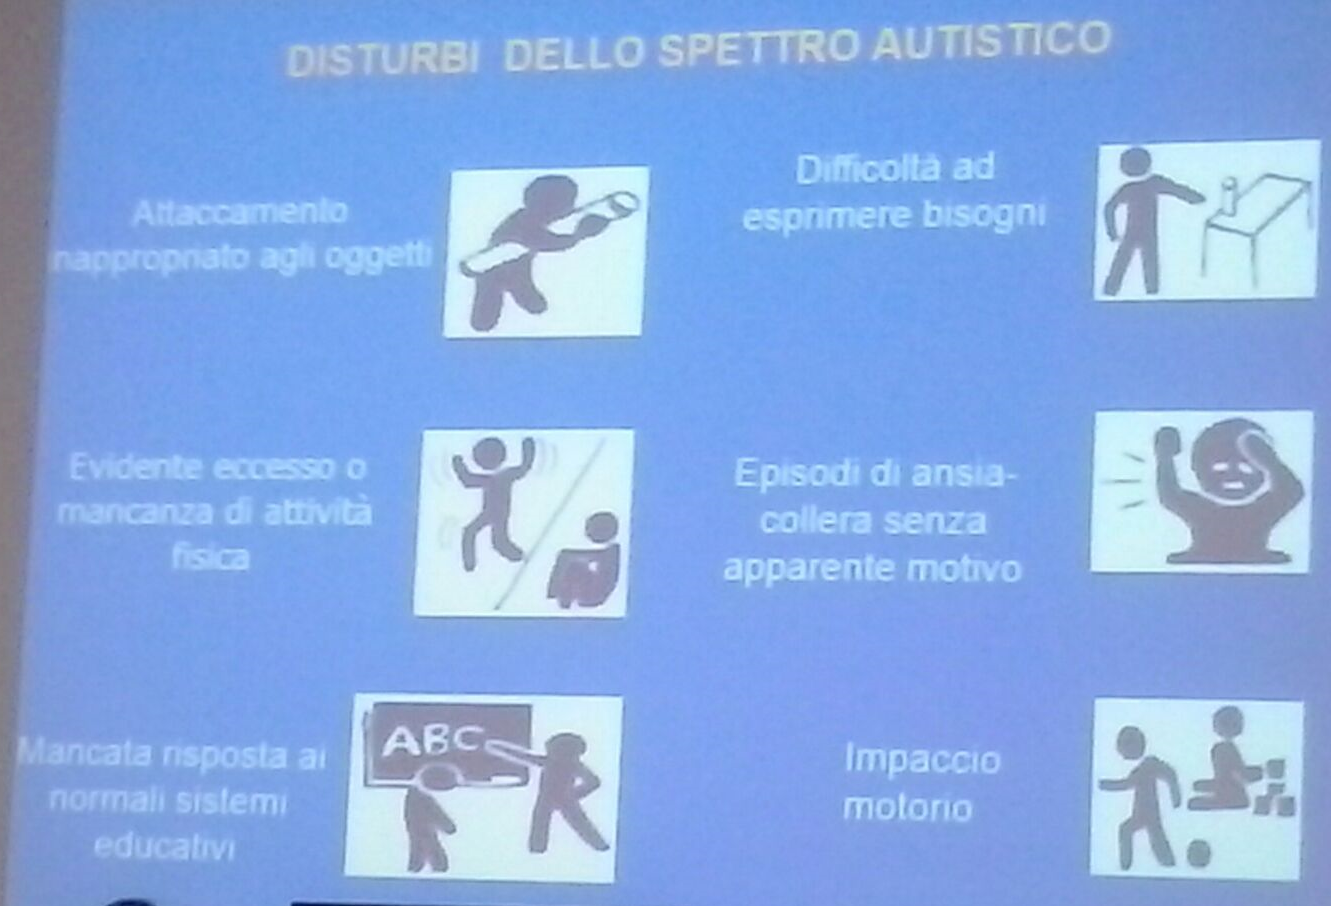
\includegraphics{media/image2.emf}

\begin{itemize}
\item
  \begin{quote}
  nigrostriatale → movimento
  \end{quote}
\item
  \begin{quote}
  tuberoinfundibolare → PRL
  \end{quote}
\item
  \begin{quote}
  mesocorticale → patogenesi della dipendenza
  \end{quote}
\item
  \begin{quote}
  mesolimbica → patogenesi della dipendenza
  \end{quote}
\end{itemize}

Quando si assume una sostanza si attiva il sistema della ricompensa (che
ha due caratteristiche: l'impatto edonico e la salienza).

Il piacere è di due tipi:

\begin{itemize}
\item
  \begin{quote}
  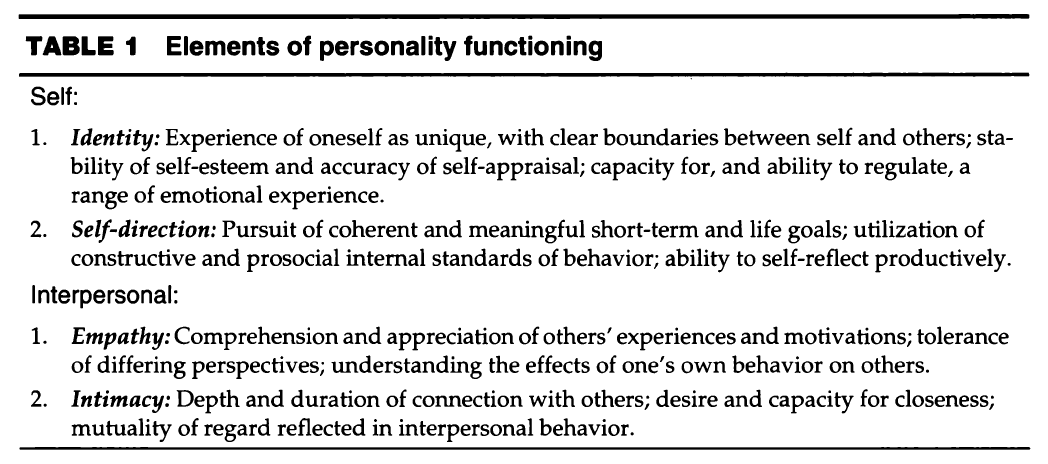
\includegraphics{media/image3.emf}anticipatorio (per il pensiero di
  fare una cosa)
  \end{quote}
\item
  \begin{quote}
  consumatorio (nel fare la cosa stessa)
  \end{quote}
\end{itemize}

Queste cose si ripercuotano sulla ricompensa, l'impatto edonico avviene
poiché i neuroni dei sistemi di reward scaricano per il piacere, quando
l'individuo capisce che una cosa può provocargli piacere anche il solo
pensiero potrà farglielo provare.

Non è tutto mediato dalla dopamina: l'impatto edonico è mediato dal GABA
e dai recettori oppioidi (ovvero il piacere consumatorio). La dopamina
media il piacere anticipatorio.

Si può avere quindi un'anedonia consumatoria o una appetitiva.

Es. gli schizofrenici hanno un'anedonia appetitiva mentre i depressi
l'hanno totale, sia consumatoria che anticipatoria.

Altro aspetto è quello del learning: l'individuo impara che una sostanza
o una situazione gli provoca piacere e successivamente cercherà di
replicare le stesse azioni per riprovarlo.

Il learning inquadra fenomeni di dipendenza come fenomeni di
apprendimento.

Anche il learning è dopamino mediato.

\emph{\textbf{Esperimento }}

In un esperimento hanno preso alcuni eroinomani e hanno chiesto loro
cosa più ricordava loro l'eroina.

Alcuni hanno risposto la siringa, altri l'odore dell'incenso (ha un
odore simile a quello dell'eroina), ecc... .

Poi li hanno muniti di tablet e ogni tanto mandavano dei messaggi che
ricordavano questi stimoli o altre cose neutre (una mela, una pera,
ecc...).

Hanno visto che le ricadute avvenivano più frequentemente dopo i
messaggi che contenevano gli stimoli appresi (la siringa per chi diceva
la siringa, l'incenso per chi diceva l'incenso e così via).

La corteccia prefrontale è coinvolta in questo processo, in quanto va ad
organizzare i comportamenti finalizzati (bilancio tra conflitti,
risoluzioni dei conflitti e desideri).

La corteccia prefrontale è divisa in varie aree:

\begin{itemize}
\item
  \begin{quote}
  parte dorso laterale (regola la working memory)
  \end{quote}
\item
  \begin{quote}
  parte orbitofrontale (media l'inibizione)
  \end{quote}
\item
  \begin{quote}
  parte ventri-mediale (media i conflitti)
  \end{quote}
\item
  \begin{quote}
  parte del cingolo anteriore (regola il dolore e il piacere)
  \end{quote}
\end{itemize}

Queste 4 parti reggono il circolo vizioso della dipendenza.

Il sistema limbico regola il piacere (nucleo accumbens regola il
piacere, l'ippocampo il ricordo del piacere e l'amigdala la salienza) e
proietta alla corteccia prefrontale.

Il learning si basa sul condizionamento operante: le punizioni e i premi
modificano la capacità di un individuo di ripete un'azione.

La capacità di valutare i pro e i contro di una determinata azione si
basa sul principio del rinforzo

\begin{enumerate}
\def\labelenumi{\arabic{enumi}.}
\item
  \begin{quote}
  positivo → l'azione mi provoca piacere e quindi la ripeto
  \end{quote}
\item
  \begin{quote}
  negativo → l'azione mi evita un dolore e quindi la ripeto
  \end{quote}
\end{enumerate}

e della punizione: evito il comportamento legato ad un danno.

Il principio dominante è la \textbf{CONTIGUITA' TEMPORALE}, ovvero è più
rilevante, e determina il comportamento, ciò che viene prima.

Un eroinomane sa che l'eroina gli fa male e che gli da degli effetti
collaterali (vomito, ascessi, malattie infettive, ecc...) ma il
desiderio di farsi una dose ed eliminare la sindrome d'astinenza è più
forte delle punizioni che verranno dopo la somministrazione.

Altro esempio, un dottore sa che il fumo fa male ma può fumare lo
stesso. Questo avviene perché il rinforzo positivo o negativo della
sigaretta vince sulla possibilità di avere un tumore fra 10 anni (ovvero
il punishment).

La realtà è però più complessa. Se si prendono due gemelli omozigoti e
si espongono all'eroina, non è detto che entrambi sviluppino una
dipendenza.

I fattori di rischio sono multipli e agiscono in modo diverso.

3 ordini di fattori di rischio:

\begin{itemize}
\item
  \begin{quote}
  \textbf{generali}: sviluppo socioeconomico dello stato, leggi e
  tassazioni, disponibilità delle sostanze, diseguaglianza tra le classi
  sociali; tutti quei fattori di pertinenza della salute pubblica.
  \end{quote}
\item
  \begin{quote}
  \textbf{sociali}: livello socioeconomico, dove si vive, dove si va a
  scuola, influenze familiari.
  \end{quote}
\item
  \begin{quote}
  \textbf{individuali}: temperamento, personalità, genetica, sesso
  (difficile capire se è l'ambiente che determina questa differenza o le
  differenze biologiche).
  \end{quote}
\end{itemize}

I fattori di rischio in ogni caso non sono deterministici, non danno
certezza.

Importante è anche il tempo d'inizio della dipendenza, se la dipendenza
inizia precocemente sarà peggiore.

I figli di soggetti che hanno una dipendenza hanno un rischio fino ad 8
volte maggiore di svilupparla, il 50\% di ciò è determinato dal carico
genetico. La genetica sta sia nel metabolismo che nell'effetto della
sostanza.

Es. Alcol deidrogenasi → i caucasici hanno più probabilità di aver
l'isotipo 1A, che fa tollerare meno l'alcol e produrre meno acetaldeide
e quindi si avranno meno effetti negativi (vomito) rispetto al tipo 1B,
comune tra gli asiatici, che porta ad un metabolismo e dipendenza
maggiore (livelli più alti di acetaldeide).

Non tutti rispondono allo stesso modo alla stessa sostanza: alcuni posso
avere più recettori di un determinato tipo rispetto ad un altro e quindi
il loro effetto sarà il predominante.

La stessa sostanza può dare effetti diversi a seconda del pattern
genetico che uno possiede.

Nella cannabis ci sono due diversi tipi di sostanze: il cannabidiolo e
THC.

Il bilancio tra queste due determina i sintomi psicotici; ciò che li
determina è il THC mentre il cannabidiolo protegge da essi.

Il problema è che alcuni nuovi tipi di marijuana sintetica coltivata
(es. skunk) tendono ad avere altissime concentrazioni di THC e basse di
cannabidiolo e questo provoca una predominanza degli effetti psicotici
in conseguenza della loro assunzione.

\textbf{\emph{INTERAZIONE GENE-AMBIENTE}}

Variabilità individuale in risposta a stimoli ambientali dipendente da
fattori geneticamente determinati.

Es. (studio su abusi infantili e personalità antisociale)

Un bambino che ha avuto un storia di abuso ha più probabilità di
sviluppare un disturbo di personalità antisociale. Non tutti i bambini
abusati però lo sviluppano.

E' stato scoperto che tale disturbo è correlato a bassi livelli di MAO
A.

Questa è stata una delle prime prove dell'interazione gene-ambiente,
dopo questo studio ce ne sono stati molti altri.

Ci sono anche altri fattori che concorrono a ciò, che sono stati
spiegati con il concetto di

correlazione (ovvero due cose che vanno di pari passo).

Ci sono tre tipi di correlazione:

\begin{itemize}
\item
  \begin{quote}
  \textbf{passiva}: i figli ereditano passivamente, senza fare niente,
  dei comportamenti.
  \end{quote}
\end{itemize}

es. figli di fumatori non solo ereditano geni che predispongono alla
dipendenza dalla nicotina ma vivranno anche in un luogo dove avranno un
accesso maggiore alle sigarette.

\begin{itemize}
\item
  \begin{quote}
  \textbf{attiva} : carattere del bambino lo porterà a mettersi in
  situazioni più o meno pericolose.
  \end{quote}
\end{itemize}

es. una persona iperattiva cede al figlio questa iperattività, che lo
porterà a ricercare ambienti a maggior rischio (viceversa per una
persona pigra).

\begin{itemize}
\item
  \begin{quote}
  \textbf{evocativa}: il temperamento del bambino evocherà una risposta
  diversa negli adulti. Un bambino felice tenderà ad evocare risposte
  più positive, mentre un bambino più scalmanato evocherà risposte più
  impulsive.
  \end{quote}
\end{itemize}

\emph{Domanda:} che differenza c'è tra impatto edonico e salienza?

\emph{Risposta}: è un concetto difficile da capire. L'impatto edonico è
la percezione del piacere, mentre la salienza è la risposta al piacere.

A due soggetti una sostanza può occupare lo stesso numero di recettori
(impatto edonico), mentre ciò che viene dato come significato soggettivo
a quella risposta è la salienza e varia tra i due soggetti. La salienza
è mediata dal learning.

La distinzione in ogni caso è abbastanza artificiosa.

\emph{Domanda}: se si resecano le vie dopaminergiche che regolano il
piacere si può eliminare il rinforzo?

\emph{Risposta}: in linea teorica si. In America negli anni 70 ci hanno
provato. Cercavano una cura per l'omosessualità, hanno impiantato degli
elettrodi a livello di queste aree per stimolare in maniera selettiva i
fasci dopaminergici, lavorando sull'apprendimento. Quando un soggetto
stava con una prostituta, per fargli apprendere quest'ultima era un
rinforzo positivo stimolavano le vie attreverso gli elettrodi.
L'esperimento però è risultato inconcludente.

Se uno fisicamente reseca le vie elimina sicuramente il piacere provato
verso la sostanza ma anche la capacità di provare piacere in generale.

\textbf{\emph{RICADUTA:}}

La dipendenza è una patologia cronica e recidivante, associata a
modificazioni cerebrali, che impatta sulla salute fisica e psicologica
del pz, oltre che sul suo ambiente (il pz non va a lavorare e vi sono
problemi all'interno della famiglia). \emph{La chiave della dipendenza è
che spinge il pz ad agire COMPULSIVAMENTE: se all'inizio la dipendenza è
volontaria, in seguito, per le modificazioni cerebrali che alterano il
self control e la capacità di resistere agli impulsi, il pz entra in
questo circuito, per cui non riesce più a smettere}.

La RICADUTA (che capita essenzialmente nel 90\% dei casi) non è colpa né
del medico né nel pz né della famiglia: \emph{è un sintomo del
disturbo.} La ricaduta avviene in modo progressivo e a essa
contribuiscono più eventi e situazioni:

\begin{itemize}
\item
  \begin{quote}
  eventi apparentemente insignificanti (cioè non necessariamente
  riconosciuti come stressanti)
  \end{quote}
\item
  \begin{quote}
  il pz può trovarsi in una situazione ad alto rischio e questa è molto
  soggettiva: ad esempio essere lasciato dalla fidanzata, passare
  davanti alla zona del mercato nero
  \end{quote}
\item
  \begin{quote}
  alla prima ricaduta si attiva il circuito di reward, per cui aumenta
  il craving e il pz arriva all'effetto di ``violazione
  dell'astinenza'': perdita del self control, sensazione di bassa
  autoefficacia e di incapacità di dirigere il comportamento; di
  conseguenza si arriva alla ricaduta completa in cui ricomincia l'uso
  della sostanza
  \end{quote}
\end{itemize}

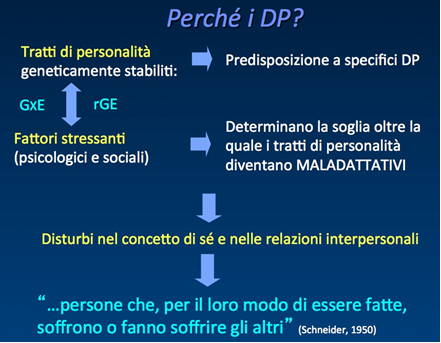
\includegraphics{media/image4.png}

\textbf{\emph{OBIETTIVI TERAPEUTICI}}

Per raggiungere gli obiettivi terapeutici è necessario agire su multipli
bersaglii: bisogna agire sulla famiglia, sul pz, sulla sua capacità di
reagire alle ricadute e di interagire con gli altri\ldots{}

Nei pz con dipendenze è molto complesso arrivare alla remissione: questa
ha percentuali bassissime, anche con la terapia sostitutiva.

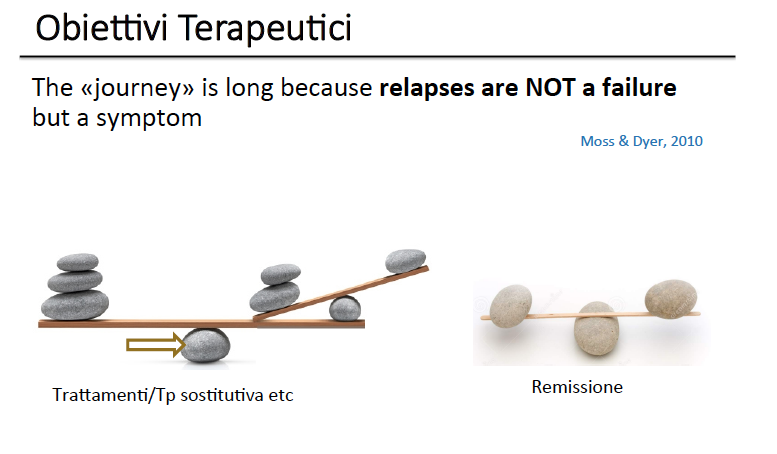
\includegraphics{media/image5.png}

\emph{COSA MINACCIA LA RELAZIONE TERAPEUTICA?}

Spesso questi pz hanno disturbi di personalità: sono disturbi pervasivi
e spesso non c'è insight del disturbo stesso (il pz non è consapevole di
averlo). In particolare si possono identificare correlazioni tra
determinati cluster e sostanze:

\begin{itemize}
\item
  \begin{quote}
  cluster B (nello specifico border e antisociale)  tendono ad
  utilizzare cocaina, eroina, alcol
  \end{quote}
\item
  \begin{quote}
  cluster A e C (evitante-ansioso)  cercano sostanze maggiormente
  sedative, meno eccitanti o socializzanti
  \end{quote}
\end{itemize}

Inoltre esiste la PERSONALITA' POST MORBOSA, che rende omogenee tutte le
diverse personalità dopo che vi è stato un disturbo da dipendenza: in
questi pz si ha un fortissimo craving ed è come se la vita iniziasse a
ruotare intorno alla sostanza, per cui essi si presentano una serie di
tratti, che sono appunto legati alla dipendenza in sé, ovvero:

\begin{itemize}
\item
  \begin{quote}
  sono intolleranti alle frustrazioni (non accettano un rifiuto)
  \end{quote}
\item
  \begin{quote}
  hanno scarsa capacità di riflettere e sono impulsivi, aggressivi
  \end{quote}
\item
  \begin{quote}
  hanno scarsa attitudine alla ``mentalizzazione'' per comprendere ciò
  bisogna considerare che vi sono almeno 3 livelli più o meno complessi
  nel vissuto:
  \end{quote}

  \begin{itemize}
  \item
    \begin{quote}
    sensazioni = in cui è difficile distinguere se proviene dall'esterno
    o dall'interno
    \end{quote}
  \item
    \begin{quote}
    emozioni = stati affettivi intensi e transitori, difficili da
    descrivere
    \end{quote}
  \item
    \begin{quote}
    sentimenti = stati affettivi duraturi e intenzionali, in cui
    l'emozione è associata ad uno specifico contenuto
    \end{quote}
  \end{itemize}
\end{itemize}

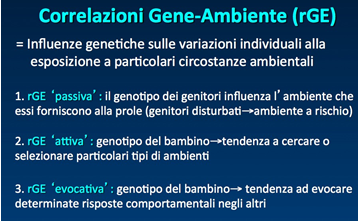
\includegraphics{media/image6.png}

Importante nelle tossicodipendenze è che si ha \emph{un'incapacità di
passare dalle sensazioni alle emozioni e ai sentimenti}: si parla di
ALESSITIMIA, l'incapacità di leggere i propri sentimenti, di
identificarli e descriverli; più spesso il pz descrive lo stato somatico
perché è più semplice.

Il pz quando si trova in una condizione di sofferenza (ad esempio il
craving) reagisce ``dissociando'': cerca di allontanare questa
condizione percepita come fastidio e ansia, di non pensarci (anziché
cercare di capire l'origine della sofferenza, di affrontare le proprie
emozioni e di strutturarle), presentando dunque una scarsa capacità di
coping, inteso come il ``cercare di adattarsi ad una situazione
stressante''.

Un esempio per capire il deficit di mentalizzazione:

P (paziente) e T (terapeuta)


\includegraphics{media/image7.png}

La pz non cerca di capire quali erano i suoi sentimenti e perché, ma
descrive le manifestazioni somatiche. È un'incapacità di astrarre, che
si manifesta in senso trasversale: è uno dei punti più importanti da
trattare in terapia.

\textbf{\emph{DIAGNOSTICA DEL SER.T (SERVIZIO TOSSICODIPENDENZE)}}

L'unico esame disponibile essenzialmente è ESAME TOSSICOLOGICO DELLE
URINE che rintraccia le sostanze più utilizzate:

\begin{itemize}
\item
  \begin{quote}
  \emph{eroina:} restano tracce nelle urine per 3-5 giorni
  \end{quote}
\item
  \begin{quote}
  \emph{cocaina:} restano tracce per 3-5 giorni
  \end{quote}
\item
  \begin{quote}
  \emph{cannabinoid}i: restano tracce per 5 giorni in caso di uso
  occasionale; se l'abuso è cronico anche per 20-40 giorni
  \end{quote}
\item
  \begin{quote}
  \emph{benzodiazepine} (BDZ): spesso il pz ha una regolare prescrizione
  per queste, inoltre cross reagiscono con diversi farmaci
  \end{quote}
\end{itemize}

Il problema è che nel 50\% delle sindromi tossicologiche non si hanno
reperti analitici di supporto per la diagnosi. Per esempio: NDMA,
ketamina, CHEM-SEX (=cocktail di GHB, ketamina, mefedrone)  in questi
casi il tossicologico è pulito: è difficile fare diagnosi, capire le
sostanze, i dosaggi, gli effetti collaterali e in conclusione come
agire.

\textbf{\emph{INTOSSICAZIONE}}

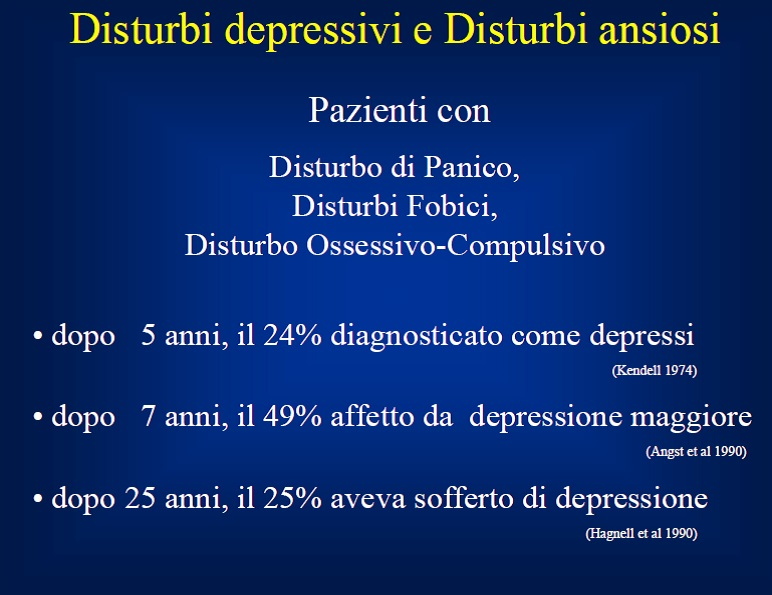
\includegraphics{media/image8.emf}

Sindrome sostanza-specifica reversibile, dovuta dalla recente assunzione
della sostanza. Importante è il criterio temporale: la sintomatologia
deve essere vicina temporalmente all'assunzione.

I sintomi non devono essere dovuti ad un'altra patologia.

Vi sono 4 sindromi tossicologiche principali, ricordando poi che spesso
un soggetto va incontro a diverse intossicazioni:

\begin{enumerate}
\def\labelenumi{\arabic{enumi}.}
\item
  \begin{quote}
  sindrome da SEDATIVI (oppiacei, bdz, barbiturici) in cui si va verso
  l'arresto cardio-respiratorio
  \end{quote}
\item
  \begin{quote}
  sindrome da STIMOLANTI (cocaina, AMF) in cui sono più aggressivi
  (soggetto, irrequieto, logorroico)
  \end{quote}
\item
  \begin{quote}
  sindrome da DISSOCIATIVI (ketamina, PCP)
  \end{quote}
\item
  \begin{quote}
  sindrome da ALLUCINOGENI (LSD)
  \end{quote}
\end{enumerate}

\emph{GLI ANTIDOTI ESISTONO PER GLI OPPIACEI E LE BDZ:}

\begin{itemize}
\item
  \begin{quote}
  NALOXONE (Narcan) per gli oppiacei
  \end{quote}

  \begin{itemize}
  \item
    \begin{quote}
    Antagonista puro
    \end{quote}
  \item
    \begin{quote}
    Emivita 30-40 min
    \end{quote}
  \item
    \begin{quote}
    Dopo risveglio il pz rischia di andare in arresto respiratorio
    perché termina l'effetto
    \end{quote}
  \item
    \begin{quote}
    Fiale da 0,2 mg, da somministrare a bolo
    \end{quote}
  \item
    \begin{quote}
    Effetto rapido
    \end{quote}
  \item
    \begin{quote}
    Si usa in caso di overdose, eventualmente per fare diagnosi di
    dipendenza: se viene somministrato esso spiazza la cocaina dai
    recettori e determina la comparsa di una grave sindrome da astinenza
    \end{quote}
  \end{itemize}
\item
  \begin{quote}
  FLUMAZENIL (Anexate) per le BDZ
  \end{quote}

  \begin{itemize}
  \item
    \begin{quote}
    Antagonista puro
    \end{quote}
  \item
    \begin{quote}
    Emivita 10 min
    \end{quote}
  \item
    \begin{quote}
    Fiale da 0,1 mg che si possono somministrare fino a quando non si
    cominciano a vedere gli effetti di stabilizzazione del quadro
    \end{quote}
  \end{itemize}
\end{itemize}

\section{\texorpdfstring{\emph{ASTINENZA:}}{ASTINENZA:}}\label{astinenza}

Le SINDROMI ASTINENZIALI sono specifiche per la sostanza e si hanno sia
quadri sia da ASTINENZA (per lo più fisica) che da INTOSSICAZIONE.

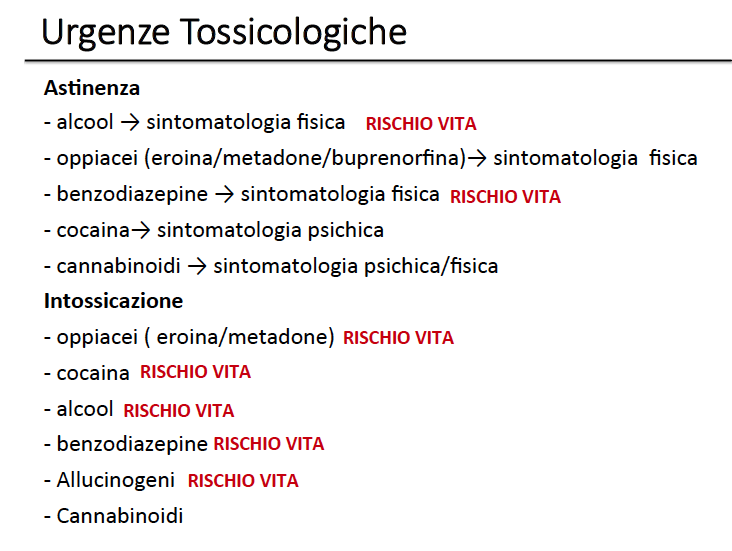
\includegraphics{media/image9.png}

Bisogna prestare attenzione alle sostanze che possono essere mortali:
tra le sindromi da ASTINENZA mortali sono le benzodiazepine e l'alcol
(in quanto l'astinenza può portare a crisi convulsive, con grande male e
coma); tra le sindromi da INTOSSICAZIONE sono gli oppiacei, la cocaina,
l'alcol, le benzodiazepine, gli allucinogeni. Le altre sostanze non sono
a rischio di vita, per esempio il metadone.

\textbf{\emph{SOSTANZE D'ABUSO:}}

alcol, caffeina, cannabis, allucinogeni, inalanti (popper), oppioidi
(eroina, morfina, ecc...), sedativo-ipnotici, stimolanti (cocaina,
amfetamine, ecc...), tabacco, ecc...

Ce ne sono sempre di nuove in quanto chi le produce ne modifica anche di
poco la struttura chimica (ad es. immettendo un gruppo ossidrilico),
come la \emph{crocodile.} Sono sostanze pericolose perché non sono
controllate e gli effetti collaterali possono essere molto gravi.

\section{CANNABINOIDI}\label{cannabinoidi}

I più frequentemente utilizzati sono Hashish (ricavato dalla resina) e
Marjuana (dalle foglie).

Costo indicativo: 1 gr = 10 \euro{}

\emph{Sintomi}

Alterazioni fisiche:

\begin{itemize}
\item
  \begin{quote}
  Apparato respiratorio: è più irritante del tabacco
  \end{quote}
\item
  \begin{quote}
  Apparato cardiovascolare: è fonte di grave stress per questo apparato
  \end{quote}
\item
  \begin{quote}
  Apparato riproduttivo: nell'uso prolungato altera il ciclo mestruale;
  riduce il testosterone quindi la libido e la fertilità
  \end{quote}
\end{itemize}

Alterazioni psichiche:

\begin{itemize}
\item
  \begin{quote}
  Ottundimento
  \end{quote}
\item
  \begin{quote}
  Alterazioni dello stato coscienza e percettive
  \end{quote}
\end{itemize}

Per quanto riguarda le alterazioni psichiche non è chiaro però se il pz
sia disturbato (con ad esempio personalità del cluster A schizoide) e di
conseguenza inizi ad utilizzare la sostanza, o viceversa è possibile che
il pz cominci ad utilizzare la sostanza e di qui sviluppi il disturbo
psicotico: secondo gli ultimi studi il \emph{rischio di sviluppare un
disturbo psicotico è 6 volte maggiore in chi utilizza la cannabis; il
rischio aumenta di altre 3 volte se si utilizzano skunk o affini (perché
aumenta THC e riduce cannabidiolo).}

Bisogna anche considerare che in questi pz che sviluppano psicosi:

\begin{itemize}
\item
  \begin{quote}
  Il 50\% non prendono la terapia farmacologica
  \end{quote}
\item
  \begin{quote}
  Pz vanno incontro alla sindrome amotivazionale (con apatia e abulia)
  \end{quote}
\item
  \begin{quote}
  Si hanno alterazioni cognitive (memoria e attenzione)
  \end{quote}
\end{itemize}

Trattamento

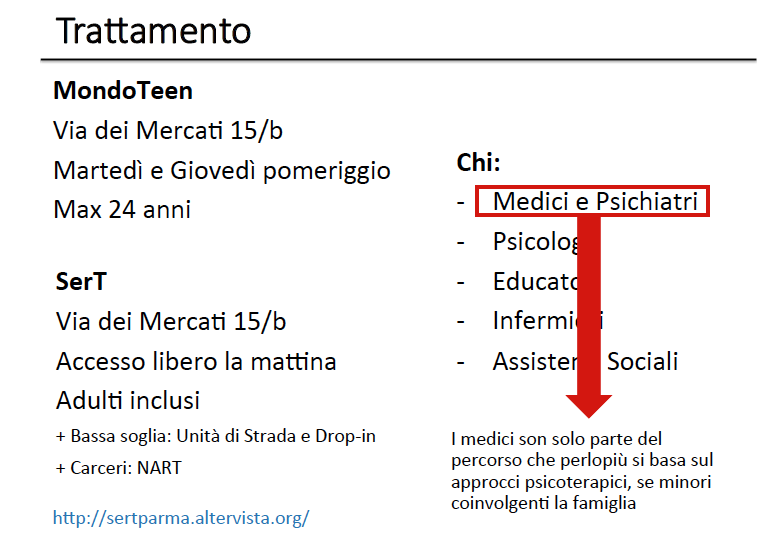
\includegraphics{media/image10.png}

\section{}\label{section}

\section{OPPIOIDI}\label{oppioidi}

Sono economici:

\begin{itemize}
\item
  \begin{quote}
  Eroina 1 dose = o,2 gr = 20\euro{}
  \end{quote}
\item
  \begin{quote}
  Metadone 100 cc (che è 5 volte la dose base) = 10-15 \euro{}
  \end{quote}
\end{itemize}

EROINA

Può essere:

\begin{itemize}
\item
  \begin{quote}
  Inalata
  \end{quote}
\item
  \begin{quote}
  Iniettata (sciolta in acido perché è una base)
  \end{quote}
\item
  \begin{quote}
  Sniffata
  \end{quote}
\item
  \begin{quote}
  Utilizzata coma supposta anale o vaginale
  \end{quote}
\end{itemize}

Fasi della dipendenza da eroina

L'eroina crea una grave dipendenza, di cui si possono riconoscere
diverse fasi:

\begin{enumerate}
\def\labelenumi{\arabic{enumi}.}
\item
  \begin{quote}
  LUNA DI MIELE
  \end{quote}

  \begin{enumerate}
  \def\labelenumii{\alph{enumii}.}
  \item
    \begin{quote}
    Il soggetto prova sensazioni molto piacevoli
    \end{quote}
  \item
    \begin{quote}
    Ne va uso salutario (astinenza lieve)
    \end{quote}
  \item
    \begin{quote}
    Si ha la percezione di poterne controllare l'uso (ma non è così)
    \end{quote}
  \end{enumerate}
\item
  \begin{quote}
  DOSI CRESCENTI
  \end{quote}

  \begin{enumerate}
  \def\labelenumii{\alph{enumii}.}
  \item
    \begin{quote}
    il soggetto ricerca gli effetti provati nella fase 1, senza mai
    poterli raggiungere (è la \emph{tolleranza farmacologica})
    \end{quote}
  \item
    \begin{quote}
    diminuisce l'aspetto euforico, aumentano il craving astinenziale e
    il bisogno della sostanza, per cui il soggetto aumenta le dosi:
    \end{quote}

    \begin{enumerate}
    \def\labelenumiii{\roman{enumiii}.}
    \item
      \begin{quote}
      rinforzo postivo = ricordo delle sensazioni sperimentate in
      precedenza con l'uso della sostanza
      \end{quote}
    \item
      \begin{quote}
      rinforzo negativo: il soggetto non vuole sperimentare i sintomi
      astinenziale
      \end{quote}
    \end{enumerate}
  \end{enumerate}
\item
  \begin{quote}
  FASE DELLA DEPRAVAZIONE (casi più gravi)
  \end{quote}

  \begin{enumerate}
  \def\labelenumii{\alph{enumii}.}
  \item
    \begin{quote}
    Soggetti sono disposti a tutto, anche ad azioni illecite, per
    procurarsi la sostanza
    \end{quote}
  \end{enumerate}
\item
  \begin{quote}
  ``PORTA GIREVOLE''
  \end{quote}

  \begin{enumerate}
  \def\labelenumii{\alph{enumii}.}
  \item
    \begin{quote}
    soggetto si rende consapevole della dipendenza  prova a
    disintossicarsi in modo autogestito  fallisce  richiede aiuto a
    Ser.T  potrà andare incontro a ricaduta (che come abbiamo detto è
    un sintomo della dipendenza)  di qui viene ricoverato in reparto,
    si rivolge al Ser.T per disintossicarsi, entra in comunità\ldots{}
    si ha un ciclo continuo!
    \end{quote}
  \end{enumerate}
\end{enumerate}

Diagnosi: ANALISI TOSSICOLOGICA DELLE URINE

La diagnosi attraverso l'esame tossicologico delle urine è molto utile,
soprattutto per gli eroinomani.

Può essere:

\begin{itemize}
\item
  \begin{quote}
  STANDARD (risultato in 3 giorni): per i casi di routine, in fase di
  accoglienza\ldots{}
  \end{quote}
\item
  \begin{quote}
  RAPIDA: è molto più sensibile, ma più costoso, da usare in certi casi
  urgenti
  \end{quote}
\end{itemize}

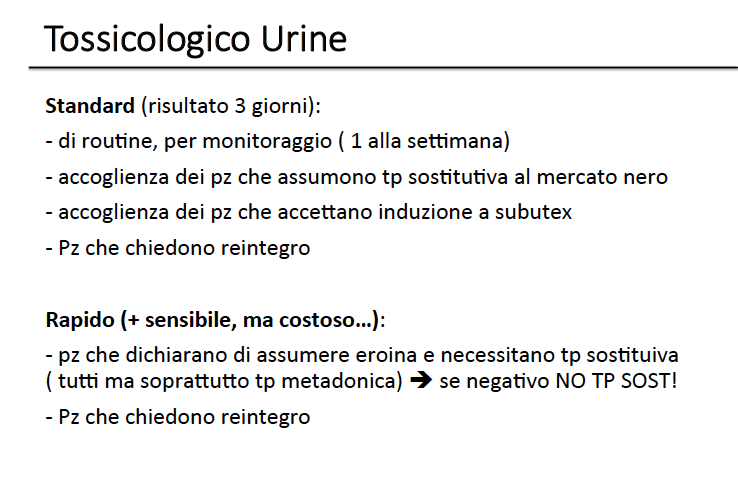
\includegraphics{media/image11.png}

Trattamento della dipendenza da eroina

Essenzialmente quando un pz arriva al Ser.T ci sono due casi possibili:

\begin{enumerate}
\def\labelenumi{\arabic{enumi}.}
\item
  \begin{quote}
  Pz assume eroina, non è mai venuto. Il tossicologico è positivo, ma ne
  assume poca. Si può provare (e ciò dipende dal pz):
  \end{quote}

  \begin{enumerate}
  \def\labelenumii{\alph{enumii}.}
  \item
    \begin{quote}
    A disintossicare il pz (c'è una sala per la disintossicazione)
    \end{quote}

    \begin{enumerate}
    \def\labelenumiii{\roman{enumiii}.}
    \item
      \begin{quote}
      Oppure si propone ricovero per la disintossicazione (più
      frequente)
      \end{quote}
    \end{enumerate}
  \item
    \begin{quote}
    A proporre la tp sostitutiva
    \end{quote}

    \begin{enumerate}
    \def\labelenumiii{\roman{enumiii}.}
    \item
      \begin{quote}
      Per eroina fumata, poca quantità (fino 1 gr/die): beprenofina
      \end{quote}
    \item
      \begin{quote}
      Dipendenza grave, da tempo: metadone
      \end{quote}
    \end{enumerate}
  \end{enumerate}
\item
  \begin{quote}
  Pz si fa di metadone  bisogna impostare la terapia sostitutiva,
  scalando la dose
  \end{quote}
\end{enumerate}

\emph{Terapia di disintossicazione (sintomatologica)}

Nella disintossicazione ci si basa su alcuni sintomi e segni
fondamentali: sono elencati nella \emph{SCALA DI COWS (Clinical Opiated
Withdrawal Scale),} che si utilizza per valutare come procede
l'astinenza e quindi trattarla. Inevitabilmente \emph{la terapia è
sintomatologica}, poiché non esiste una terapia perfetta.

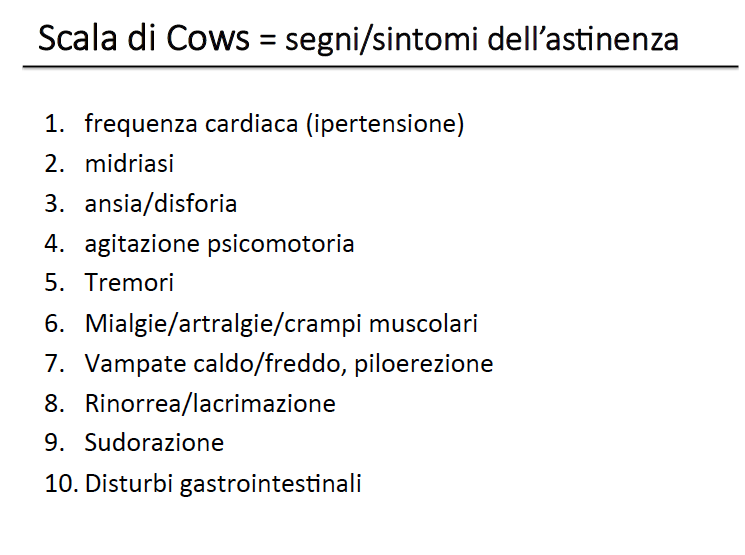
\includegraphics{media/image12.png}

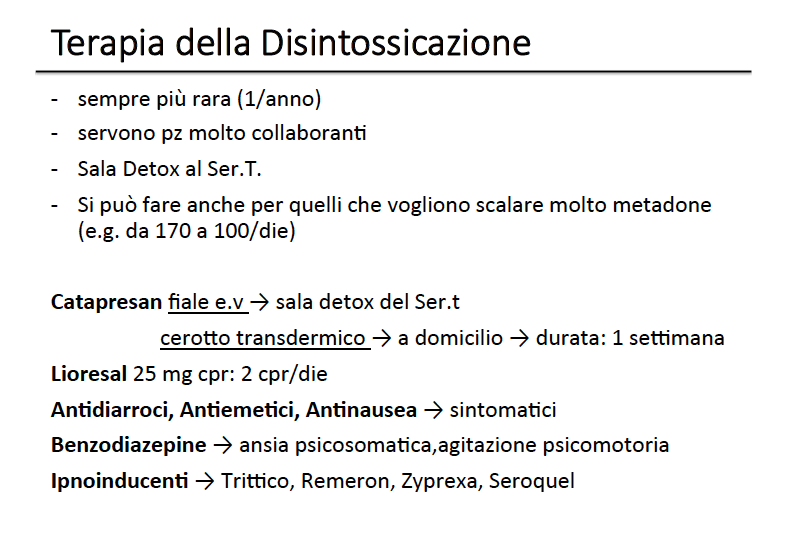
\includegraphics{media/image13.png}

In particolare:

\begin{itemize}
\item
  \begin{quote}
  Catapresan
  \end{quote}
\item
  \begin{quote}
  Mioresal = miorilassante
  \end{quote}
\item
  \begin{quote}
  Antidiarroici e antiemetici
  \end{quote}
\item
  \begin{quote}
  Bdz per ansia e irrequietezza
  \end{quote}
\end{itemize}

DOMANDA: I sintomi da spiazzamento e da astinenza sono gli stessi? R:
Sì! (e sono quelli della scala di Cows).

METADONE

\begin{itemize}
\item
  \begin{quote}
  È un agonista puro con lunga emivita, quindi l'astinenza ci mette
  molto ad insorgere e copre i sintomi di craving
  \end{quote}
\item
  \begin{quote}
  Non si ha picco ematico, per cui i pz se lo fanno endovena, ma è
  estremamente tossico!
  \end{quote}
\item
  \begin{quote}
  Viene utilizzato come terapia sostitutiva nella disintossicazione:
  \end{quote}

  \begin{itemize}
  \item
    \begin{quote}
    30 mg/die è un quantitativo tossico per chi non utilizza questa
    sostanza: si consideri però che nei soggetti dipendenti si usano
    anche 200 mg!!
    \end{quote}
  \item
    \begin{quote}
    Oltre i 100 mg è importante fare la lettura del QTC
    \end{quote}
  \item
    \begin{quote}
    Si scala circa 5-10 gr alla settimana, molto lentamente perché si
    presenta il craving!
    \end{quote}
  \item
    \begin{quote}
    È metabolizzato da CYP3A4: importante \emph{l'interazione
    farmacologica}
    \end{quote}
  \end{itemize}
\end{itemize}

\begin{quote}
In particolare:

Fluvoxamina  inibisce CYP3A4  aumenta livelli plasmatici metadone

Carbamazepina  induce CYP3A4  riduce livelli plasmatici metadone
\end{quote}

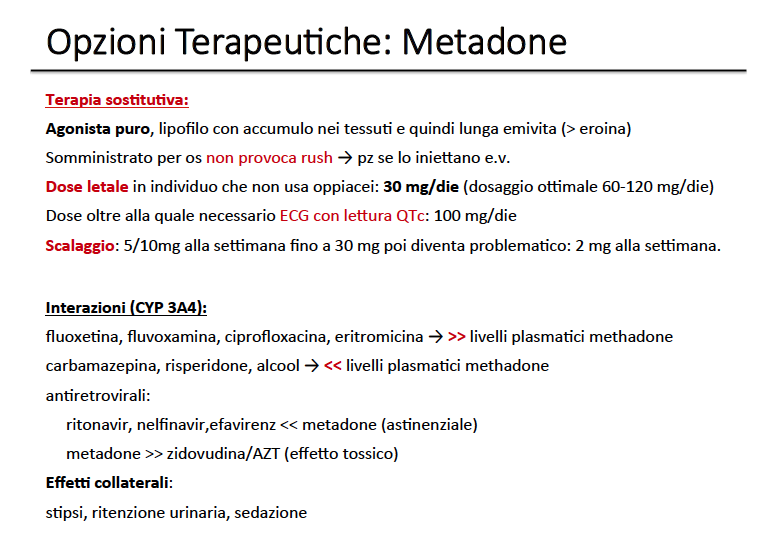
\includegraphics{media/image14.png}

PRO e CONTRO del Metadone nella terapia sostitutiva:

il professore ha praticamente letto la slide

PRO:

\begin{itemize}
\item
  \begin{quote}
  pz non deve essere in astinenza
  \end{quote}
\item
  \begin{quote}
  ``piace più del subotex'' (vedi dopo)
  \end{quote}
\end{itemize}

CONTRO:

\begin{itemize}
\item
  \begin{quote}
  può portare ad overdose  si ha Narcan come antidoto, ma potrebbe
  essere necessario somministrarlo per più giorni perché il metadone ha
  una lunga emivita
  \end{quote}
\item
  \begin{quote}
  si sviluppano sintomi astinenza, che durano per molto tempo perché ha
  un'emivita lunga  soprattutto le alterazioni del sonno restano anche
  per più di un mese
  \end{quote}
\end{itemize}

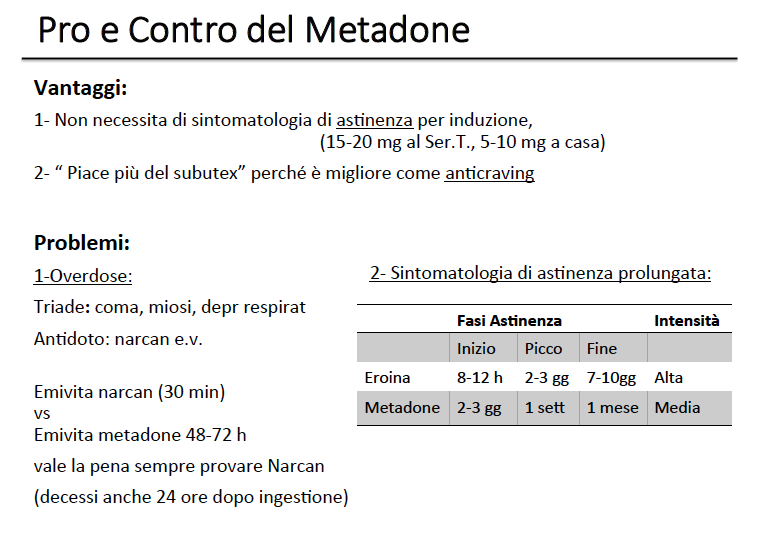
\includegraphics{media/image15.png}

Affido

Nella terapia sostitutiva il pz può recarsi al Ser.T ogni giorno per
prendere la dose, oppure viene fatto un accordo per la gestione autonoma
della terapia (l'affido): viene data la dose necessaria al pz ad esempio
per una settimana, il quale la assumerà a casa. Questo da un lato è un
rischio, dall'altro porta il pz ad avere maggiore fiducia in sé, proprio
perché viene responsabilizzato. L'affido ha dunque un forte significato
cognitivo-comportamentale.

Durante l'affido si può andare incontro a diversi scenari possibili, per
esempio che il pz arrivi e richieda una dose maggiore perché riferisce
di dover andare in vacanza: in questo caso si può affidare una dose
maggiore, ma bisogna verificare la veridicità di ciò che il pz riferisce
(ad esempio se deve andare in vacanza si richiede di vedere documenti
che lo testimonino); altra situazione possibile è che il pz riferisca di
avere finito la dose: il medico può decidere se effettuare o meno il
``\emph{reintegro}''. Ciò può essere concesso a patto che il pz si rechi
tutti i giorni al Ser.T per prendere la dose (essenzialmente si
ricomincia da capo il processo, l'affido viene temporaneamente sospeso).
Si tenga predente che fatto che abbia esaurito la terapia potrebbe
essere legato a cause diverse:

\begin{itemize}
\item
  \begin{quote}
  Misuso = i pz se lo fanno ev, ad esempio per mitigare la fase crash
  post utilizzo di cocaina
  \end{quote}
\item
  \begin{quote}
  Diversione = il pz ha venduto la dose
  \end{quote}
\item
  \begin{quote}
  Dosaggio insufficiente = il pz ha assunto davvero una dose maggiore,
  ma per tenere sotto controllo il craving (la dose è effettivamente
  insufficiente, devo aumentare il dosaggio)
  \end{quote}
\end{itemize}

SUBUTEX

\emph{Subutex (buprenorfina) -- sempre per la terapia sostitutiva}

\begin{itemize}
\item
  \begin{quote}
  Agonista \emph{parziale} recettori mu: c'è l'effetto tetto
  \end{quote}
\item
  \begin{quote}
  Ha affinità elevata per i recettori degli oppiacei (spiazza tutto)
  \end{quote}
\item
  \begin{quote}
  Antagonista kappa: minor disforia e anedonia
  \end{quote}
\item
  \begin{quote}
  Emivita lunga = 3 giorni
  \end{quote}
\item
  \begin{quote}
  Vantaggi: non c'è rischio di overdose e migliora la disforia
  \end{quote}
\item
  \begin{quote}
  Svantaggi: non si ha il rush, di conseguenza il pz può continuare a
  farsi di eroina, ma va in overdose perché non arriva al rush; inoltre
  per usare il subutex il soggetto deve essere ``pulito'' da almeno 12
  ore e presentare i sintomi astinenziali. \emph{Per verificare ciò si
  danno 2 mg di subotex}: se si osserva una sintomatologia da
  spiazzamento in breve tempo allora significa che il pz si era fatto di
  eroina (che a causa del farmaco viene spiazzata rapidamente), se
  invece il pz presenta alcuni sintomi astinenziali e questi con la
  somministrazione di 2 mg di subotex rimangono tali o migliorano
  lievemente, allora il pz è effettivamente in astinenza  allora è
  possibile somministrare altri 1-2 mg di subotex (al massimo si arriva
  a 6 mg) fino a che non si vede il controllo della sindrome
  astinenziale stessa. \emph{In conclusione è importante distinguere i
  sintomi da spiazzamento (rapidi e intensi) da quelli da astinenza (più
  lenti)}
  \end{quote}
\end{itemize}

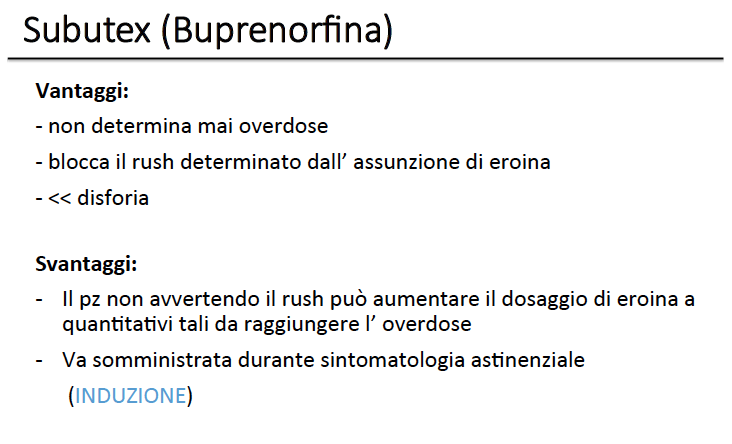
\includegraphics{media/image16.png}

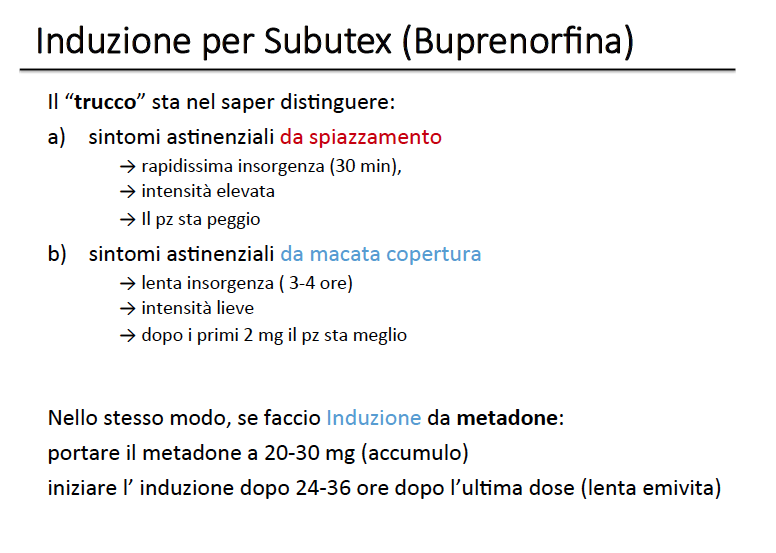
\includegraphics{media/image17.png}

\section{COCAINA}\label{cocaina}

\begin{itemize}
\item
  \begin{quote}
  Generalmente viene sniffata o fumata
  \end{quote}
\item
  \begin{quote}
  Costo: 1 gr = 100 \euro{} (costosa); crack: 1 pepita 0,2 g = 15
  \euro{}
  \end{quote}
\item
  \begin{quote}
  Speed ball = cocaina + eroina (per lo più iniettato ev)
  \end{quote}
\end{itemize}

Consumo

Il problema della cocaina \emph{induce rapidamente la tolleranza} (in
particolare all'euforia), già alla prima assunzione: ciò porta i
soggetti, soprattutto alle prime assunzioni, al BINGE (abbuffata), in
cui continuano a farsi tutto il giorno (arrivando anche fino a 5 gr di
cocaina), al fine di continuare a provare le sensazioni di HIGH
(euforia), per poi arrivare ad essere completamente spossati; smettono
di assumere la sostanza e passano alla fase CRASH-DOWN.

Fasi dell'astinenza

\begin{enumerate}
\def\labelenumi{\arabic{enumi})}
\item
  \begin{quote}
  CRASH: inizia subito dopo il binge o il consumo della sostanza e dura
  alcuni giorni. Il soggetto è demoralizzato, depresso, stanco.
  \end{quote}
\item
  \begin{quote}
  ASTINENZA: dura da 2-10 settimane, il soggetto ricerca la sostanza, il
  craving eè fortissimo e compaiono le ideazioni suicidarie (la vita non
  ha senso senza la sostanza)
  \end{quote}
\item
  \begin{quote}
  ESTINIZIONE INDEFINITA (di tempo indefinito): il soggetto è un
  consumatore occasionale di cocaina (oppure si è disintossicato) e sta
  bene, ma può avere episodi di craving per stimolazione ambientale (per
  esempio comincia il craving passando davanti ad un luogo dove si
  faceva di cocaina)
  \end{quote}
\end{enumerate}

Intossicazione

Le manifestazioni internistiche dell'intossicazione sono legate
all'iperattivazione di tutte le catecolemine, la cui liberazione è
indotta dalla sostanza stessa.

Ricordate in particolare la MIDRIASI della pupilla, a differenza degli
eroinomani che presentano la MIOSI.

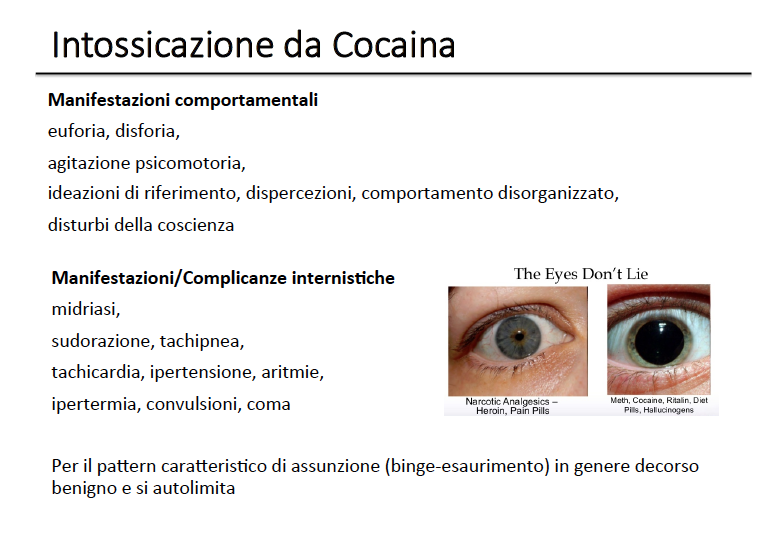
\includegraphics{media/image18.png}

\emph{ALCOL E COCAINA:} spesso utilizzati insieme, perché l'alcool rende
più socievoli nella fase high e mitiga la fase crash  il problema è che
sono \emph{competitivi nel metabolismo} e formano il
\emph{coca-etilene}, composto tossico e con maggiore emivita. In questo
caso l'intossicazione è difficile da trattare, perché si hanno due
sostanze che agiscono con azione opposta su SNC.

\section{ALCOL}\label{alcol}

NB: il professore riferisce che per l'esame, quindi dal punto di vista
psichiatrico, è importante sapere complicanze come ad esempio il delirio
di gelosia, più che tutte le complicanze a livello di sistema
gastroenterico o SN.

Cenni Storici:

Nel 1849 Magnus Huss, medico svedese, coniò il termine ALCOLISMO in un
libro che conteneva la classificazione sistematica dei danni fisici e
mentali derivanti dalle dipendenze. Nel 1935 fu fondata l'anonima
alcolisti: la dipendenza da alcol venne considerata una malattia.

Epidemiologia

Il Italia circa il 20\% della popolazione beve alcolici in maniera
inadeguata e di questi 1/3 risulta alcol dipendente. Il consumo sta
aumentando in giovani donne.

Costituisce la prima causa di morte tra i giovani europei, provocando 59
000 decessi per anno. Rappresenta il terzo problema sanitario dopo le
malattie cardiache e neoplastiche. La più frequenti di morte in questi
pazienti sono: SUICIDIO, COMPLICAZIONI CARDIOVASCOLARI, EPATICHE, MORTI
PER LA GUIDA IN STATO DI EBBREZZA.

Eziopatogenesi

L'alcol determina danni sia diretti sia indiretti, ma la loro entità
dipende dalla quantità ingerita e dalla durata di abuso. Importanti sono
la Razza, la tolleranza congenita, il substrato personologico e
l'ambiente.

Effetti fisiologici dell'alcol

L' Etanolo (famiglia alcoli, CH3-CH2-OH) è contenuto nelle bevande
alcoliche. Viene assorbito solo per il 10\% nello stomaco e tutto il
resto dal tratto digiuno ileale, in meno di un'ora con una velocità che
dipende:

-Dal volume alcolico contenuto nella bevanda

-Dall'alimentazione ( stomaco vuoto e alimenti con tanti lipidi
aumentano )

-Dalla presenza di additivi (CO2)

Una volta assorbito, essendo idro-liposolubile, attraversa facilmente le
membrane cellulari e diffonde in tutti i tessuti, con un picco
plasmatico tra i 30 minuti e le 2 ore dall'assunzione.

Viene metabolizzato per il 90\% dal fegato con processi di ossidazione,
mentre il resto viene escreto immodificato dai reni ed espirato dai
polmoni.

Il fegato metabolizza l'etanolo in maniera differente in base ad ETA',
SESSO, RAZZA, CONDIZIONI MEDICHE ASSOCIATE, TERAPIE PSICOTROPE
CONCOMITANTI, CONDIZIONE ORGANO STESSO, e lo fa principalmente grazie a
due enzimi: l'alcol deidrogenasi ( ADH ) e l'aldeide deidrogenasi.

ADH trasforma l'etanolo in acetaldeide ( tossico ) che poi viene ridotto
in acido acetico dall'acetaldeide deidrogenasi. ADH ha variabilità
genetica e razziale, per esempio gli indiani d'America e gli orientali
hanno una bassissima tolleranza.

Altri sistemi minori di metabolizzazione alcolica sono: SISTEMA
MICROSOMIALE DI OSSIDAZIONE DELL'ETANOLO (MEOS) e la CATALASI (ruolo
accessorio)

Definizione

Nel DSM IV TR vengono distinti:

1)DISTURBI DA USO DI ALCOL -\/-\textgreater{} DIPENDENZA E ABUSO

2) DISTURBI INDOTTI DA ALCOL -\/-\textgreater{} INTOSSICAZIONE ALCOLICA,
delirium DA ASTINENZA, DEMENZA PERSISTENTE, DISTURBO AMNESTICO
PERSISTENTE, DISTURBO PSICOTICO CON DELIRI E/O ALLUCINAZIONI, DISTURBI
DELL'UMORE, DISTURBI D'ANSIA, DISFUNZIONE SESSUALE, DISTURBI DEL SONNO E
NON ALTRIMENTI SPECIFICATI.

Correlati biologici dell'alcolismo

Strutture e circuiti implicati nei meccanismi di abuso, dipendenza e
craving sono principalmente: L'AREA VENTROTEGMENTALE (regione del
mesencefalo con neuroni dopaminergici), il NUCLEO ACCUMBENS (area dello
striato che riceve proiezioni dall'area tegmentale ventrale) e la
corteccia prefrontale.

Modulazioni neurotrasmettitoriali

-SISTEMA SEROTONINERGICO: sembra facilitare recettori 5HT1B,2 e 3 pre e
post sinaptici; il trasportatore SERT risulta interessato nella
patologia da abuso alcolico.

-SISTEMA GABAERGICO: l'etanolo è il grado di modificare la conformazione
del recettore GABAA (modificazione espressione genica con aumento
subunità alfa e diminuzione subunità alfa6) , con una riduzione della
trasmissione GABAergica. In soggetti che abusano si è vista una
riduzione della densità e della distribuzione dei recettori del GABA.

-SISTEMA GLUTAMATERGICO: l'etanolo ha una elevata affinità per NMDA
recettore il quale inibisce il flusso ionico. La somministrazione
cronica di etanolo determina una up-regulation dei recettori NMDA nella
corteccia e nell'ippocampo e determina in condizioni di astinenza un
aumentato release di glutammato e neurotossicità. ( la ketamina ha un
effetto analogo ). L'effetto euforizzante può essere attenuato dal
pretrattamento con antagonisti del recettore M degli oppioidi (
naltrexone ).

-SISITEMA DOPAMINERGICO: la delezione del recettore D2 porta una
tendenza alla riduzione delle dipendenza di alcol mentre una delezione
di D4 e di DAT una supersensitività all'alcol. Si è vista infatti una
riduzione dei recettori D2 D3 e trasp. DAT negli studi post mortem degli
alcolisti.

MODULAZIONE DEI MECCANISMI DI TRADUZIONE DEL SEGNALE

Adenilciclasi e proteina kinasi a sono coinvolte. Dopo esposizione
CRONICA c'è una diminuita risposta dell' AC (neurotrasmettitore indotta
ed eterologa e della PKA), mentre l'esposizione ACUTA determina un
potenziamento dell'attività di AC.

NEUROIMAGING ha dimostrato una progressiva riduzione della sostanza
grigia in sede temporale antero-superiore, una riduzione del metabolismo
cerebrale.

Disturbi da uso di alcol

1)ABUSO DI ALCOL: (per il DSM 4) modalità patologica dell'uso di alcol
che porta a menomazione o a disagio clinicamente significativi, come
manifestato da una o più delle seguenti condizioni (ricorrenti entro un
periodo di 12 mesi )

- uso ricorrente della sostanza che determina un'incapacità di adempiere
ai principali compiti connessi con il ruolo sul lavoro, a scuola o a
casa

- ricorrente uso della sostanza in situazioni fisicamente rischiose (es
guidando un' automobile )

- ricorrenti problemi legali correlati alle sostanze ( arresti per
violenze o guida in stato di ebbrezza )

- uso continuativo della sostanza nonostante persistenti o ricorrenti
problemi sociali o interpersonali causati o esacerbati dagli effetti
della sostanza (violente liti coninugali in stato di ebbrezza, abuso
contro i bambini )

I sintomi NON soddisfano i criteri per la dipendenza da alcol o da altre
sostanze

2) DIPENDENZA DA ALCOL: è è caratterizzata da prove evidenti di
tolleranza o da sintomi di astinenza.Caratterizzata (per il DSM4 ) da 3
o più delle seguenti condizioni:

- tolleranza

- astinenza

- la sostanza è assunta in quantità maggiori o per periodi più lunghi,
rispetto a quanto previsto dal soggetto, il desiderio di assumerla è
persistente e i tentativi per ridurre l'uso sono infruttuosi

- la ricerca della sostanza richiede una grande quantità di tempo speso
nella sua ricerca e nella sua assunzione

- l'interruzione o la riduzione di importanti attività socio-lavorative
o ricreative a causa dell'uso della sostanza

- nonostante la consapevolezza della presenza di problemi fisici,
psichici e sociali legati al'abuso, l'utilizzo della sostanza permane

Quadro clinico con sintomi COGNITIVI, COMPORTAMENTALI, FISIOLOGICI. Il
paziente avverte un forte desiderio di bere e spende la maggior parte
del suo tempo per ricercare la sostanza e per smaltirne gli effetti e la
sua assunzione continua anche dopo l'insorgenza di manifestazioni
psicologiche o fisiche avverse. Si assiste a un progressivo decadimento
morale sociale e fisico. Il paziente minimizza l'abuso di alcol e la
presenza di disturbi somatici e mentali ritardando cosi l'intervento dei
familiari e il riconoscimento della dipendenza. L'abuso cronico di alcol
provoca un decadimento generale fino allo sviluppo di veri e proprio
quadri di deterioramento mentale ( demenza alcolica ). La gravità
dipende dalla durata dell'abuso e dal tipo di risorse messe in atto per
combatterlo. Nelle prime fasi non si rilevano segni fisici né
alterazioni degli esami di laboratorio. Successivamente insorgono
disturbi fisici: anoressia, nausea, vomito, GERD, diarrea, palpitazioni,
insonnia, amenorrea, impotenza, poliuria, irritabilità, nervosismo,
vuoti di memoria, riduzione capacità mnesiche. Il paziente comincia a
trascurarsi con: alitosi, atassia, parola impastata, epatomegalia,
facies tipica ( rinofima ed eritema persistente con o senza
teleangectasie); poi insufficienza epatica pancreatica e renale: ascite,
ittero, dolore addominale, intolleranza ai cibi, ematemesi, melena, calo
ponderale, stanchezza, eritema palmare, angiomi aracniformi, varici
esofagee, atrofa testicolare, ginecomastia e contratture di dupuytren).

Nelle forme croniche possono essere presenti sintomi psichiatricie
neurologici con sindrome da astinenza ( convulsioni, allucinosi e
delirium), manifestazioni psicotiche (paranoia, allucinazioni, deliri,
in assenza di compromissione del sensorio), neuropatie periferiche e
deficit cognitivi.

Non rare le miopatie e le cardiomiopatie, comuni anche le cadute con
conseguenti fratture toraciche ed ematomi subdurali. Conduce a una
situazione di emarginazione che interferisce con la possibilità di
recupero. Il DSM IV consente di codificare il decorso della dipendenza
distinguendolo in:

-remissione iniziale completa/remissione iniziale parziale

-remissione protratta completa/remissione protratta parziale, e di
specificare se l'entità del disturbo è lieve, moderata o grave e se
associato o no a dipendenza fisica, cioè se sono o no soddisfatti i
criteri della tollernza e dell'astinenza.

Disturbi MENTALI indotti dall'alcol

-INTOSSICAZIONE ALCOLICA: è una sindrome reversibile dovuta all'
ingestione recente di alcol, con comportamenti mal adattativi
clinicamente significativi o modificazioni psicologiche (es.
comportamento sessuale o aggressivo inappropriato, labilità dell'umore,
difetto nelle capacità critiche, compromissione nel funzionamento
sociale e lavorativo) che si sviluppano durante o poco dopo l'ingestione
di alcol. Ci possono essere pronuncia indistinta, mancanza di
coordinazione, nistagmo, deficit dell'attenzione o della memoria, stupor
e coma. ( tutti non dovuti a una condizione medica generale o ad altri
disturbi mentali). L'intossicazione è spesso associata ad abuso o
dipendenza da alcol. L'alcol provoca ipereccitabilità neuronale con
disinibizione e impulsività sul piano affettivo e comportamentale.

Il quadro clinico: i primi disturbi compaiono a un tasso alcolemico
compreso fra 0,3 e 0,5 g/l con irritabilità, spinta a parlare,
compromissione della critica e del giudizio, sensazione di benessere
fisico e di forza, ideazione accelerata, le percezioni sono vivaci,
mimica e gestualità accentuate. Sul piano fisico: vasodilatazione,
sudorazione, ipersecrezione gastrica; poi impaccio dei movimenti,
atassia e disartria. Con un' alcolemia tra 1 e 2 g /l si manifestano,
atassia, sindrome cerebellare cinetica e statica, sindrome vestibolare,
incoordinazione, stato confusionale e coma (\textgreater{}3g/l). Con
un'alcolemia tra 4 e 7 g/l compare stato comatoso con ipotermia,
depressione respiratoria e areflessia fino al decesso. Lo stato di
ebbrezza dura circa 12 ore residuando malessere, astenia, cefalea con
umore depresso o disforico. La memoria degli avvenimenti e conservata.

-INTOSSICAZIONE DA ALCOL IDIOSINCRASICA : non è riconosciuta come
categoria diagnostica ufficiale nel DSM4. Si sviluppa rapidamente per
l'assunzione di quantità di alcol insufficienti a indurre intossicazione
nella maggior parte degli altri individui. Fattori predisponenti sono:
danno cerebrale organico e specifici aspetti personologici come il
disturbo antisociale. La sintomatologia varia da individuo a individuo;
dall'agitazione psicomotoria con atteggiamenti pantoclastici a deliri
con sfondo persecutorio o di gelosia.

-ASTINENZA ALCOLICA:sono le manifestazioni cliniche e bioumorali che
colpiscono l'alcolista alla sospensione o alla drastica riduzione di
alcol. I sintomi si sviluppano da 6 a 48 ore dopo la sospensione. Il
classico segno è il tremore che può essere accompagnato da sintomi
psicotici ( deliri e allucinazioni ), da crisi epilettiche e da sintomi
del delirium tremens.

Il TREMORE ``a battito d'ala'' compare 6-8 ore dopo, quelli PSICOTICI E
PERCETTIVI 8-12 ore, le CRISI EPILETTICHE 12-14 e il DELIRIUM TREMENS
(D.T) da 3 a 7 giorni dopo. Alcune volte però può manifestarsi
direttamente con il D.T. Altri sintomi sono irritabilità, nausea,
vomito, aumento attività del simpatico ( ansia, ipervigilanza,
sudorazione, arrossamento del volto, midriasi e aumento PA). Tutti
questi sintomi non devono essere causati da una situazione medica
generale e non devono essere spiegati con un altro disturbo mentale.
Questa \emph{sindrome da astinenza} può anche essere scatenata da traumi
cranici, infezioni o malattie. Si distinguono 4 categorie cliniche ad
intensità crescente:

\begin{enumerate}
\def\labelenumi{\arabic{enumi})}
\item
  \begin{quote}
  La \emph{SAA}( sindrome da astinenza alcolica) \emph{minore}( tremore
  alcolico ): si manifesta entro 6-24 ore con tremore a battito d'ala (
  brividi a grandi scosse), ansia,vomito,nausea e insonnia, e si risolve
  in 2-3 giorni. E' quella che si riscontra più frequentemente.
  \end{quote}
\item
  \begin{quote}
  \emph{SAA maggiore}( allucinosi alcolica ). Entro 10 -- 72 ore
  colpisce prevalentemente i maschi con allucinazioni vivide e
  persistenti, con tremori diffusi a tutto il corpo, vomito, sudorazione
  e ipertensione. (L'esordio è prevalentemente notturno, può o meno
  seguire al delirium e consiste in allucinazioni visive con
  obnubilamento dello stato di coscienza) Nell'allucinosi alcolica sono
  presenti allucinazioni uditive a contenuto terrifico nel contesto di
  uno stato di coscienza conservato-\/-\textgreater{} percezione senza
  oggetto con insight della percezione, cioè il soggetto è consapevole
  che si tratti di una allucinazione; frequenti sono le idee di
  riferimento e l'elaborazione di un sistema delirante vero e proprio.
  Il paziente si dimostra orientato nel tempo e nello spazio, inquadra i
  deliri e le allucinazioni nel suo ambiente reale e può anche ricordare
  lucidamente gli avvenimenti le sensazioni e le idee dell'episodio
  psicotico. Vi è apprensione e paura spesso associate a rabbia e
  depressione, ci possono essere comportamenti di evitamento o di difesa
  con condotte autolesive quando ci sono anche idee di indignità e di
  colpa. Il decorso varia da 5 giorni ad un mese, e talvolta può avere
  un andamento cronico, in questo caso i fenomeni dispercettivi perdono
  la risonanza affettiva e divengono più egodistonici-\/-\textgreater{}
  il pz comprende che la situazione è dovuta all'astinenza da alcol.
  \end{quote}
\item
  \begin{quote}
  \emph{Convulsioni d'astinenza} ( rum fits ): sono crisi di grande
  male, 12-24 ore dopo la sospensione dell'alcol in circa il 5\% dei
  pazienti. Nel 60\% le crisi sono multiple, e nel 3\% si giunge ad un
  male epilettico. Il quadro in genere si risolve il 2-5 giorni la
  risoluzione può essere con un sonno profondo oppure con regressione
  dei sintomi in 2-3 settimane. Nel 30-40\% dei pazienti si sviluppa
  delirium tremens.
  \end{quote}
\item
  \begin{quote}
  \emph{Delirium tremens} (DT) (sutton 1813). Il meccanismo
  eziopatogentico non appare chiaro. Colpisce circa l'1-2\% dei soggetti
  e può rappresentare l'evoluzione del cosiddetto tremore alcolico e
  dell'epilessia alcolica. L'insorgenza è notturna e correlata a una
  brusca sospensione da alcol, in genere in bevitori cronici da almeno 5
  anni, 1-3 giorni dopo la sospensione. Spesso esiste un pre-delirium
  con irritabilità, rapide oscillazioni del tono dell'umore, ansia,
  tremore agli arti e ai muscoli facciali, febbricola e torpore,
  insonnia iniziale e centrale con fasi di sonno inquieto e incubi.
  Delle volte emerge senza prodromi dopo un trauma, un intervento
  chirurgico, disidratazione o malattie infettive. All'esame obiettivo
  il paziente è CONFUSO, DISORIENTATO E ANGOSCIATO dall'esperienza
  allucinatoria. CLINICAMENTE:
  \end{quote}
\end{enumerate}

\begin{itemize}
\item
  \begin{quote}
  A) turbe psichiche: stato confusionale con disorientamento nel tempo e
  nello spazio, agitazione e insonnia, illusioni, allucinazioni visive (
  microzoopsie = piccoli animali sul corpo che fanno ribrezzo e
  macrozoopsie= grossi animali nello spazio esterno, minacciosi) e
  uditive a contenuto minaccioso e disturbi dell'ideazione con temi
  deliranti frammentari o in genere sorretti dalle alterazioni
  percettive (delirio occupazionale = imitazione dei gesti quotidiani
  per ristrutturare il continuum vitale interrotto dalla psicosi.
  L'attenzione è focalizzata sul contenuto allucinatorio e il pensiero è
  frantumato nei vissuti deliranti, il contenuto è incoerente e
  contraddittorio. La memoria è alterata durante l'episodio e ( con
  variabilità) dopo l'episodio.
  \end{quote}
\item
  \begin{quote}
  B) disturbi neurologici: iperreflessiaosteotendinea e tremori a grandi
  scosse diffusi ed evidenti agli arti al capo e alla lingua. Nella fase
  di esordio: cefalea, nistagmo posizionale, midriasi, atassia,
  disartria. Comparsa di riflessi patologici ( suzione, prensione e
  grasping) indicano grave compromissione cerebrale. Il sonno prolungato
  è un indice prognostico positivo e le crisi epilettiche possono
  complicare il quadro.
  \end{quote}
\item
  \begin{quote}
  C) sintomi somatici associati: sempre iperidrosi, e se associata a
  vomito o diarrea può dare grave disidratazione. Spesso: tremori,
  tachicardia, tachipnea, ipertermia, oliguria, iperemia congiuntivale e
  ipotensione. Broncopolmonite ab ingestis e il collasso
  cardiocircolatorio possono complicare il quadro.
  \end{quote}
\end{itemize}

\begin{quote}
Il DT può essere prevenuto se il paziente è adeguatamente monitorato e
trattato. L'indice di mortalità varia dal 5 al 15\%. Le cause di morte
sono insufficienza respiratoria e le aritmie cardiache.

-DISTURBO AMNESICO ALCOLICO: ridotta capacità di apprendere nuove
informazioni o l'incapacità a richiamare informazioni precedentemente
apprese che causa una significativa riduzione del funzionamento sociale
o lavorativo. Esiste una forma TRANSITORIA ( meno di un mese ) o di
LUNGA DURATA ( più di un mese ) e i sintomi devono essere correlati
all'uso di alcol. Si manifesta in persone che hanno assunto grandi
quantità di alcol per molti anni. Quadro clinico: la capacità di
acquisire nuovo materiale è ridotta con un'amnesia anterograda e
disorientamento nel tempo, l'amnesia retrograda è di varia intensità. La
percezione e le altre funzioni cognitive sono di solito integre. ( se
prevalgono i disturbi cognitivi meglio una diagnosi di demenza o di
delirium ). L'alterazione della memoria può essere associata a
modificazioni della personalità: apatia, agitazione, amichevoli o
accondiscendenti. La confabulazione può essere significativa. Questi
soggetti non hanno una chiara consapevolezza della loro condizione. La
prognosi è variabile ma almeno all'inizio il recupero può essere quasi
completo.

-VUOTI DI MEMORIA ( BLACKOUT ): non sono inclusi del DSM 4, anche se è
un sintomo di intossicazione comune. Consistono in singoli episodi di
amnesia anterograda, in associazione a un'intossicazione alcolica. Si ha
un deficit specifico della memoria a breve termine con incapacità di
richiamare gli aventi accaduti nei 5-10 minuti precedenti. Le altre
funzioni cognitive sono conservate. I pazienti temono di avere
inconsciamente fatto del male a qualcuno o di essersi comportati in modo
imprudente. Si sa solo che l'alcol blocca il consolidamento delle nuove
tracce mnesiche in ricordi, un processo in cui si pensa siano coinvolti
l'ippocampo e le strutture del lobo temporale a esso collegate.

-PARANOIA ALCOLICA ( DELIRIO DI GELOSIA ) : nel DSM 4 non è menzionata
da sola, ma è inserita all'interno delle manifestazioni psicotiche
indotte da alcol con deliri e allucinazioni. Non è un segno
patognomonico ma è molto frequente. Nasce come ``dubbio'' poi diventa
certezza dell'infedeltà assoluta e impermeabile a ogni confronto con la
realtà. La convinzione deriva da prove certe e inconfutabili ottenute
dal controllo continuo esercitato sul partner, spiando, pedinando,
controllando la corrispondenza e gli effetti personali. Delle volte
cerca di far ammettere la colpa all'altro chiedendo ammissioni,
confessioni, estorcendole con il ricatto, la coercizione e la violenza
fisica. Aumentano il sospetto il rifiuto del coniuge di avere rapporti
sessuali, la perdita della posizione socio-familiare, la diminuzione del
desiderio e della potenza sessuale per l'effetto dell'alcol. Colpisce
più i maschi in età avanzata e può avere un decorso cronico e
indipendente dalle condotte di abuso.

-DEMENZA: 10\% dei pazienti con abuso protratto. Dopo Alzheimer e
disordini cerebrovascolari è la più frequente causa di demenza. Vi è un
aumentato volume dei ventricoli e un'atrofia corticale ma non è ancora
chiara la patogenesi. Si ritiene però difficile separare gli effetti
tossici dell'abuso alcolico dal danno del SNC causato dalla
malnutrizione, dai traumi multipli, e dagli effetti dannosi sul SNC
della disfuzione di altri organi. Il DSM 4 afferma che possa provocare:
disturbi cognitivi multipli, con deficit della memoria, delle funzioni
corticali superiori e modificazioni dei tratti di personalità. Queste
sono irreversibili.
\end{quote}

Disturbi FISICI indotti dall'alcol

\emph{SISTEMA GASTROINTESTINALE}

\begin{quote}
ESOFAGO E STOMACO: l'assunzione acuta causa infiammazione di mucosa
esofagea e gastrica, ci può essere dolore in sede epigastrica,
microemorragie e anoressia. Nei forti bevitori cronici lacerazione della
mucosa nella giunzione gastro esofagea ( s. di malloryweiss), se
associata a vomito. La maggior parte di questi sono reversibili, ma
l'assunzione cronica può causare complicanze come varici esofagee e
atrofia gastrica.

INTESTINO TENUE: interferisce con l'assorbimento delle vitamine del
gruppo B e di altre sostanze, in acuto ci possono essere lesioni
emorragiche dei villi duodenali e diarrea ( aumento motilità per
irritazione ). Deficit di tiamina e folati.

PANCREAS: determina pancreatite acuta che può assumere un andamento
cronico, causata da un'attivazione intrapancreatica degli enzimi
digestivi, con digestione delle membrane cellulari, proteolisi, edema,
emorragia interstiziale, danno vascolare e necrosi. Vi è un meccanismo
di liberazione di amine vasoattive e bradichinine responsabili di
vasodilatazione, aumento permeabilità ed edema con pancreatite acuta che
può andare incontro a cronicizzazione. È presente dolore addominale,
diarrea e vomito. Vi è un aumento delle amilasi sieriche, leucocitosi,
iperglicemia ipocalcemia e occasionalmente ittero.

FEGATO: l'alcol assorbito giunge subito al fegato, come fonte di
energia. Si verifica un accumulo di NADH, con una gluconeogenesi
inadeguata, accumulo di lattato e ridotta ossidazione degli acidi
grassi, con uno stoccaggio di grasso nelle cellule epatiche= steatosi.
In un indivudo sano queste alterazioni sono ancora reversibili, ma se vi
è un'esposizione ripetuta ci può essere epatite alcolica e cirrosi. Le
tre principali forme di epatopatia sono: steatosi epatica, epatite
alcolica, cirrosi.

\emph{La steatosi epatica:} è un processo reversibile e NON rappresenta
una condizione predisponente per epatite e cirrosi alcolica.

\emph{L'epatite alcolica:} è una lesione infiammatoria con infiltrazione
di leucociti, necrosi epatocellulare, ialinosi alcolica, ed è la
principale causa predisponente per la cirrosi. La guarigione causa
infatti fibrosi che sovverte l'architettura e porta allo sviluppo di
\emph{cirrosi:} caratterizzata da una fibrosi diffusa con presenza di
noduli rigenerativi. Il connettivo circonda i vasi portali e periportali
riducendo il numero di epatociti, lasciando spazio ai fibroblasti con
una riduzione del volume e della funzione d'organo che diventa di
consistenza lignea. I segno sono tardivi con emorragie digestive,
ascite, ed encefalopatia epatica. A livello ematico vi è aumento delle
transaminasi, gamma gt, fosfatasi alcalina, leucocitosi polinucleare e
VGM aumentato.

\emph{CUORE:} la carenza di vitamine causa una fibro-necrosi delle
cellule cardiache con aumento di volume e cardiopatia dilatativa
congestizia.

\emph{SISTEMA EMATOPOIETICO:} nell'abuso occasionale si trova anemia
macrocitemica, nelle deficienza di acido folico, reticolocitopenia e
iperplasia midollare. Si riscontra anche leucocitopenia e alterazioni
della funzionalità dei neutrofili e trombocitopenia; con un aumento di
emorragia ed infezioni.

\emph{SISTEMA NERVOSO CENTRALE}:

\emph{SINDROMI DI WERNICKE E DI KORSAKOFF:} classici disturbi amnesici,
la prima acuta e la seconda cronica. La S. di Wernicke è totalmente
reversibile, la seconda ha una remissione completa solo nel 20\% dei
casi. Sono correlate a carenze vitaminiche del complesso B e in primis
della tiamina, dovute al malassorbimento e alla scorretta alimentazione.

° LA SINDROME DI WERNICKE= ( encefalopatia alcolica) è un disturbo
neurologico acuto con paralisi del retto laterale dell'occhio e della
coniugazione laterale dello sguardo, atassia nella marcia e alterazioni
mentali fino a stato confusionale completo. A livello oculare vi è un
riflesso pupillare più rallentato e anisocoria. Se non trattata può
sfociare nella °SINDROME AMNESICA CRONICA CI KORSAKOFF= quadro amnestico
confabulatorio con amnesia ante e retrograda con un gravissimo
disadattamento, spesso sono presenti alterazioni di attenzione e
concentrazione con difficoltà a spostare l'attenzione su diversi
compiti, difficoltà nella fluenza verbale e nella labilità
visuo-spaziale. La confabulazione è tipica delle fasi precoci e serve
per mascherare le amnesie. I disturbi del comportamento sono frequenti
con apatia, indifferenza ma conservata reattività all'ambiente e
capacità di comprendere e risolvere problemi. All'anatomia patologica si
riscontra un danno al tronco dell'encefalo e del diencefalo a livello
periventricolare con grosso interessamento dei corpi mammillari e altre
strutture. La somministrazione di tiamina è fondamentale soprattutto
nello stato iniziale prima della condizione cronica.

\emph{MALATTIA DI MARCHIAFAVA BIGNAMI:} colpisce etilisti maschi di età
adulta, e si associa a epatopatia e malnutrizione. Può essere acuta con
convulsioni e coma o subacuto simile a una condizione di ebbrezza
cronica. ci sono alterazioni delle funzioni frontali o demenza
progressiva che evolve in alcuni anni, clinicamente abbiamo:
irritabilità, aggressività, violenza verbale e fisica, manifestazioni
psicotiche, apatia, disartria, afasia, aprassia, anomalie del
comportamento sessuale e rallentamento motorio. Più raramente
spasticità, emiparesi e insufficienza sfinterica. Può essere reversibile
o avere un'evoluzione cronica se non trattata. Si è vista una simmetrica
distruzione delle fibre mieliniche del corpo calloso e interessamento
delle commessure anteriore e posteriore. Le cause sembrano essere
metaboliche soprattutto a livello temporoparieto occipitale.

\emph{DEGENERAZIONE CEREBELLARE DA ALCOL:} forma di atassia cerebellare,
tipica delle forme croniche, con degenerazione delle cellule del
purkinje. Atassia degli arti inferiori e instabilità tronco.

\emph{MIELINOSI PONTINA CENTRALE:} degenerazione focale simmetrica della
mielina centropontina. Vi è paralisi bulbare spastica e tetraplegia che
possono anche determinare la morte. Il pz è in perenne ebrezza alcolica.

\emph{ATROFIA CORTICALE CEREBRALE:} frontale, e ampliamento degli spazi
dei ventricoli laterali e del terzo

\emph{SISTEMA NERVOSO PERIFERICO}

\emph{POLINEUROPATIA periferica} : è una progressiva degenerazione della
guaina mielinica, con interessamento sia motoria che sensitivo con una
modalità centripeta, che parte dagli arti inferiori, possono essere
coinvolti il nervo vago e il nervo frenico.

\emph{RISCHIO DI CANCRO:} è la seconda causa di morte negli alcolisti e
la frequenza dei carcinomi è 10 volte superiore che nella popolazione
normale. Soprattutto a carico di esofago, cardias, stomaco, fegato e
pancreas. Nelle donne anche le neoplasie mammarie.
\end{quote}

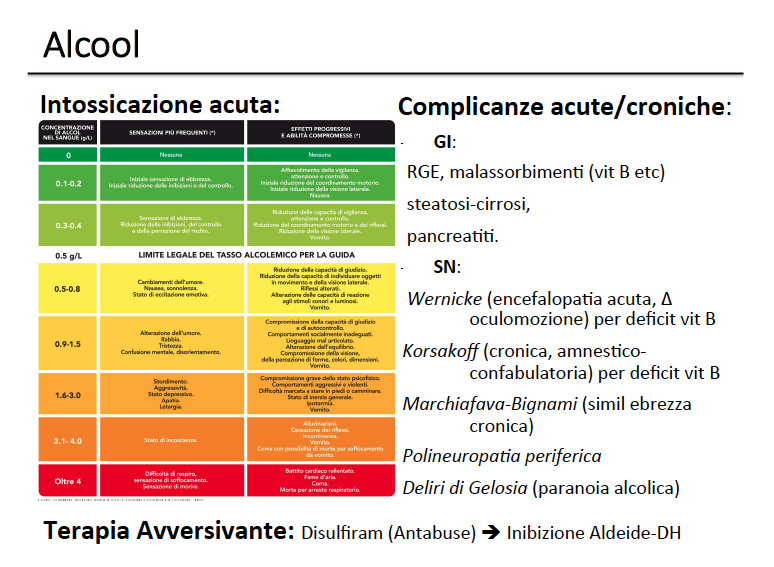
\includegraphics{media/image19.png}

\textbf{\emph{TRATTAMENTI DELLE DIVERSE CONDIZIONI DI ABUSO DI ALCOL:}}

\textbf{\emph{Trattamento farmacologico:}}

REAZIONI TOSSICHE: l' alcolemia sopra i 200/250 mg-ml è da considerarsi
un'emergenza medica e psichiatrica, con un controllo adeguato di
ventilazione, P.A, funzione cardiaca, bilancio elettrolitico,
metabolismo glucidico, da trattare in un reparto di rianimazione. Da
valutare, condizioni mediche associate come patologie infettive e
traumatismi ( ematomi subdurali ) oppure l'assunzione di altre sostanze
d'abuso. Se si sospetta uso di oppiacei  naloxone 0,4 mg ev o im.

ABUSO CRONICO: dipendenza e astinenza. Nella dipendenza è cruciale
pianificare la progressiva riduzione dell'assunzione plurima e
quotidiana d'alcol, con strategie terapeutiche farmacologiche e non.
Farmaci usati sono disulfiram ( entabuse) che inibisce l'acetaldeide
deidrogenasi ( terapia avversivante) : i soggetti, se assumono bevande o
alimenti contenenti anche minime quantità di alcol provano un grave
malessere (viene a loro fornita una lista di tutti gli alimenti vietati)
e acamprosato. Le benzodiazepine sono utili come terapia di supporto
dell'astinienza

CRAVING: pazienti possono beneficiare dal trattamento con SSRI. Tra i
farmaci in grado di modulare la funzione serotoninergica centrale hanno
sperimentato il buspirone( agonista 5HT1A ) e la ritanserina (
antagonista 5-HT2A-C ) ma senza grossi risultati. Il disulfiram è un
inibitore dell'aldeide deidrogenasi e se il paziente dovesse assumere
alcol si manifesta flushing cutaneo, cefalea pulsante, sudorazone
profusa, ipertensione, dispnea, ma raramente ci sono complicanze. Gli
effetti collaterali sono: alitosi, dermatite allergica, neuropatie
periferiche, epatopatie. Il disulfiram inibisce anche la
dopamina-beta-idrossilasi, e in pazienti psicotici o schizofrenici la
sua assunzione deve essere valutata per l'aumento di dopamina centrale.

ASTINENZA: è diversa in base alla gravità del quadro. Lieve media
gravità: controllo della sintomatologia comportamentale e psichica ( in
assenza di complicanze o emergenze ). Utilizzate benzodiazepine a lunga
emivita ad alti dosaggi impiegate in quadri di ansia acuta per le quali
si alza il dosaggio fino all'interruzione dei sintomi. Il diazepam se vi
sono convulsioni. Le benzodiazepine possono talora complicare il quadro
clinico dell'alcolismo per la possibilità d'abuso. Esiste anche una
doppia sindrome di astinenza benzodiazepine -- alcol con una maggiore
frequenza e intensità dei sintomi di tipo neurovegetativo e
psicomotorio. Anche la carbamazepina è stata utilizzata come
neuroprotettore e per le complicanze convulsive. L'acamprosato ( analogo
strutturale del gaba ) si è dimostrato efficace per prevenire i sintomi
dell'astinenza dopo la disitonsicazione alla dose di circa 900/1200
mg/die, il principale effetto collaterale è la diarrea.Utilizzate anche
integrazioni vitaminiche per le sindromi dell'SNC.

DELIRIUM TREMENS: ricovero in terapia intensiva. Anamnesi. Con
interventi terapeutici per le sindromi organiche da alcole volti a
correggere il deficit vitaminico ( complesso B e PP ) e le eventuali
alterazioni della glicemia e gli squilibri elettrolitici. Per i sintomi
comportamentali benzodiazepine, di solito diazepam( 5-10mg ) ripetendo
le dosi fino alla sedazione ( attenzione alla funzione respiratoria )

SINDROME AMNESTICA PERSISTENTE:( E SINDROME WERINCKE KORSAKOFF) alte
dosi di tiamina. Nella S. di Wernickegia basse dosi ( 1-2 mg) possono
far regredire i sintomi oculari, 50-100 mg endovena può determinare la
risoluzione del quadro clinico in alcune settimane. La correzione con
tiamina deve SEMPRE precedere l'apporto di glucosio perché la carenza di
tiamina determina un'alterata risposta al carico di glucosio introdotto.

\textbf{\emph{Terapie non farmacologiche}}:

un approccio monodimensionale di questo tipo non è praticabile e
l'integrazione di una terapia farmacologica è probabilmente la strategia
più concretamente effettuabile. Ruolo fondamentale è quello della
PSICOTERAPIA COGNITICO COMPORTAMENTALE ( per la dipendenza ). Anche
TERAPIE DI GRUPPO E INTERVENTI PSICOEDUCATIVI possono essere utili. Il
coinvolgimento del nucleo familiare può essere utile laddove il problema
delle spinte a comportamenti di dipendenza alcolica richieda una forte
allenza terapeutica. Altri modelli che coinvolgono la famiglia sono il
family functioning ( con focus sul funzionamento generale del gruppo
familiare, del quale l'alcolismo è solo un'espressione di un disagio più
esteso e complesso ) e dal behavioural family model ( basato
sull'introduzione di rinforzi positivi d'interazione a livello del
coniuge o degli altri membri del nucleo familiare ) e poi gli ALCOLISTI
ANONIMI (nati nel 1935 negli usa) organizzazioni composte da alcolisti
che si basano sull'aiuto reciproco allo scopo di mantenere la propria
sobrietà e consentire agli altri di raggiungerla attraverso un programma
di recupero spirituale, mirato alla ricostruzione della personalità
sulla base di valori e di principi fondamentali per ka vita di ogni
essere umano, con frequenti e regolari incontri dove il nuovo arrivato
mette il gruppo a conoscenza della proprio condizione di alcolista e i
membri più anziani, raccontanto la propria esperienza con l'alcol e la
strada percorsa per uscirne, forniscono un supporto emozionale evitando
l'isolamento sociale.

\textbf{\emph{DOMANDE DEGLI STUDENTI:}}

(ndr il professore risponde leggendo rapidamente le slide, oltre a
quelle riportate sotto ve ne sono altre, ma in generale si tratta di
argomenti di curiosità, come riferisce Lui stesso; il professore
\emph{riferisce poi di avere inserito delle slide sull'ipotesi
dopaminergica della schizofrenia, trattata nella lezione precedente})

Il trattamento del gioco d'azzardo patologico (gambling)

Il trattamento è principalmente cognitivo-comportamentale: viene
effettuato un inquadramento finanziario, poi sono indicati la
psicoterapia individuale (per gestire i trigger ad esempio passare
davanti alle macchinette) e gruppi di mutuo aiuto. Si fa un tutoraggio
finanziario per cui al pz viene dato 1 euro al giorno o carte prepagate
con 50\euro{} alla settimana, mirando a guidare il pz verso il controllo
finanziario.

La terapia psichiatrica è indicata solo in caso di episodi depressivi o
ideazioni suicidiarie secondari alla crisi finanziaria.

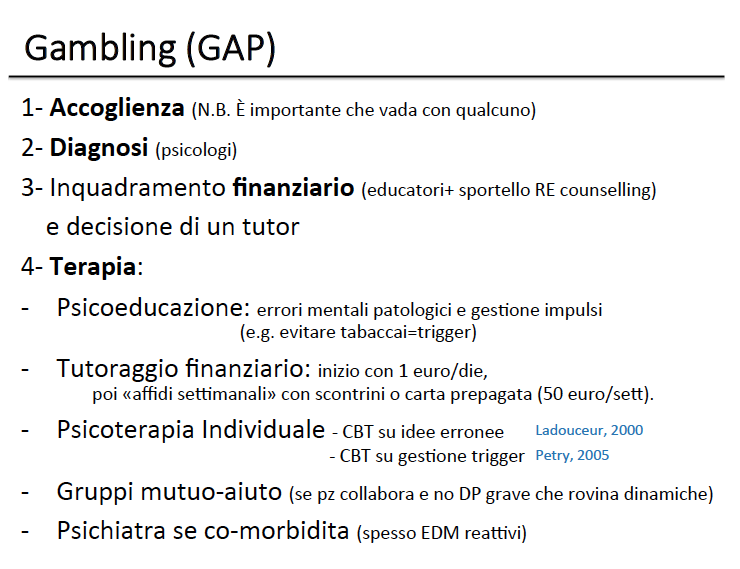
\includegraphics{media/image20.png}

Le dipendenze in ambito sanitario

Le dipendenze più frequenti sono alcol, BDZ, oppioidi,

La prevalenza non è molto maggiore rispetto alla popolazione generale.

I più a rischio sono gli studenti di medicina e tra gli specializzanti
sono gli anestesisti. Tra i medici le cinque categorie che vanno
incontro all'abuso sono i medici di medicina generale, gli anestesisiti,
gli psichiatri, i medici di medicina interna e di urgenza.

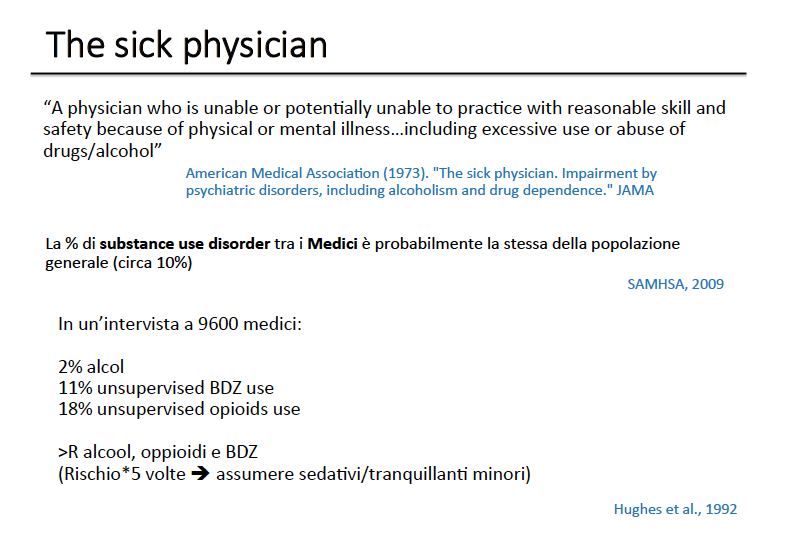
\includegraphics{media/image21.png}

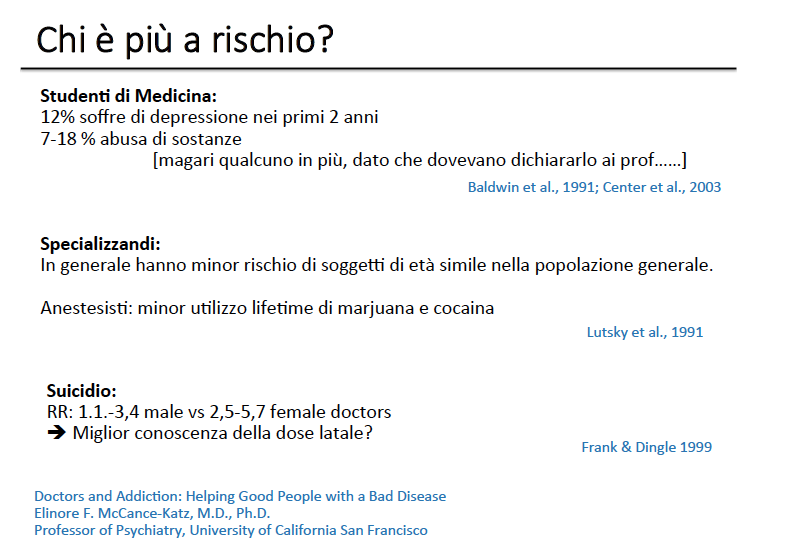
\includegraphics{media/image22.png}

La dipendenza da lavoro:

Frequente in ambito accademico

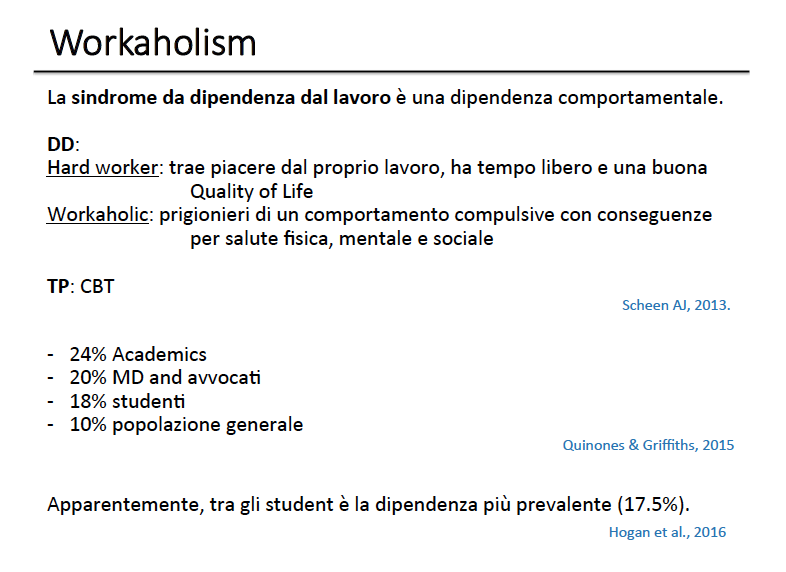
\includegraphics{media/image23.png}

Lsd e neurotossicità

Vi sono studi contrastanti: solo in alcuni casi si hanno flashback e
allucinazioni persistenti fino ad un anno o per più tempo.

\emph{LSD agisce su due livelli:}

\begin{itemize}
\item
  \begin{quote}
  allucinazioni visive a livello della corteccia visiva
  \end{quote}
\item
  \begin{quote}
  alterazioni del sé a livello paraippocampale  il soggetto è
  dissociato dalla realtà e percepisce la realtà in modo diverso, il
  significato cambia  prinicipio della percezione delirante
  \end{quote}
\end{itemize}

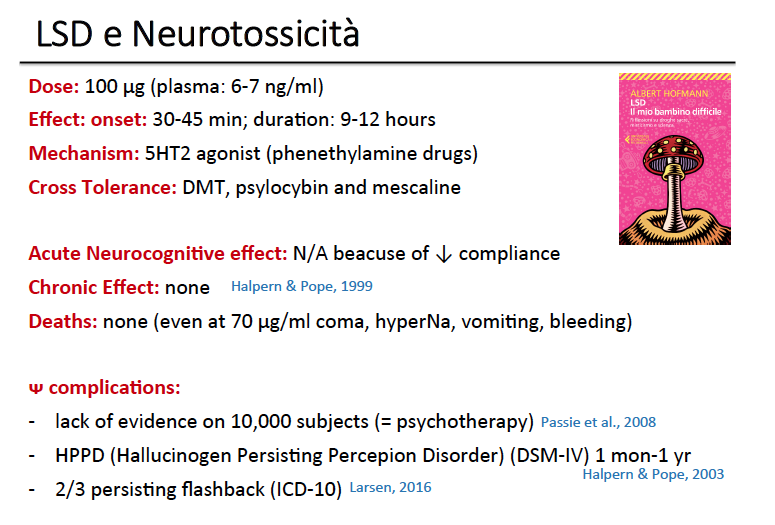
\includegraphics{media/image24.png}

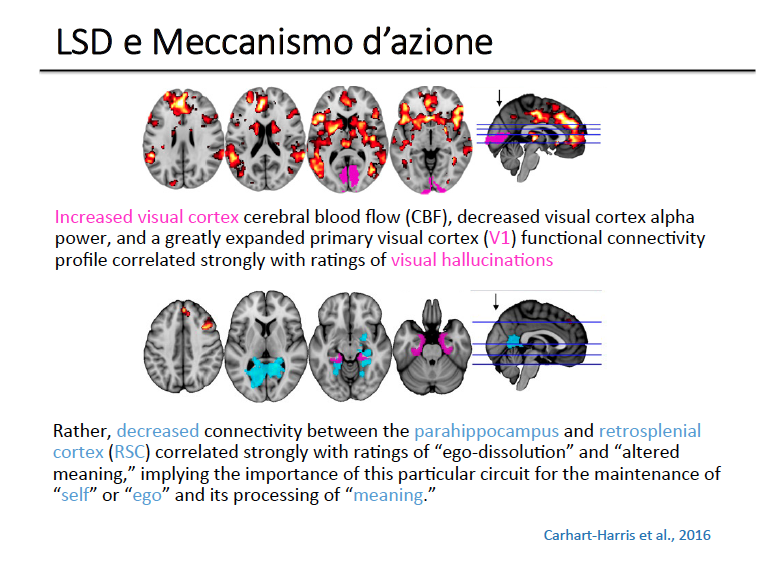
\includegraphics{media/image25.png}

\end{document}
